\documentclass{article}

\usepackage{blindtext}
\usepackage[utf8]{inputenc}

\usepackage{graphicx,fancyhdr,amsmath,amssymb,amsthm,subfig,url,hyperref}
\usepackage{algorithm}
\usepackage{algpseudocode}
\usepackage{booktabs}
\usepackage{float}
\restylefloat{table}
\usepackage[margin=1in]{geometry}
\usepackage{amsthm}
\usepackage{multirow}
\usepackage{enumitem}
%\usepackage{enumerate}
\usepackage[normalem]{ulem}
\usepackage{accents}
\usepackage{thm-restate}
\usepackage{physics}
\usepackage[numbers]{natbib}

\usepackage{todonotes}

\newcommand{\specialcell}[2][c]{%
  \begin{tabular}[#1]{@{}c@{}}#2\end{tabular}}

%----------------------- Macros and Definitions --------------------------

%%% FILL THIS OUT
\newcommand{\studentname}{Oliver Hinder}
\newcommand{\suid}{ohinder}
%%% END

\newcommand{\ubar}[1]{\underaccent{\bar}{#1}}

 
%\usepackage{algorithm,algcompatible,amssymb,amsmath}

%\renewcommand{\COMMENT}[2][.5\linewidth]{%
%  \leavevmode\hfill\makebox[#1][l]{//~#2}}
%\algnewcommand\algorithmicto{\textbf{to}}
%\algnewcommand\RETURN{\State \textbf{return} }

% If {a} then b End
\algnewcommand{\IfR}[1]{\State\algorithmicif\ #1\ \algorithmicthen}
\algnewcommand{\EndIfR}{\unskip\ \algorithmicend\ \algorithmicif}


\renewcommand{\theenumi}{\bf \Alph{enumi}}

\theoremstyle{plain}
\newtheorem{theorem}{Theorem}
\newtheorem{assumption}{Assumption}
\newtheorem{example}{Example}


\newtheorem{claim}[theorem]{Claim}
\newtheorem{observation}[theorem]{Observation}

\newtheorem{lemma}[theorem]{Lemma}
%\newtheorem{assume}[assume]{Assumption}
%\newtheorem{example}[example]{Example}


\newtheorem{corollary}[theorem]{Corollary}
\newtheorem{definition}[theorem]{Definition}
\newtheorem{remark}[theorem]{Remark}
\newtheorem{fact}[theorem]{Fact}
%\declaretheorem[name=Theorem,numberwithin=section]{thm}
%\declaretheorem[name=Lemma,numberwithin=section]{lem}


\newcommand{\matStart}{\begin{pmatrix}}
\newcommand{\matEnd}{\end{pmatrix}}

\fancypagestyle{plain}{}
\pagestyle{fancy}
\fancyhf{}
\fancyhead[RO,LE]{\sffamily\bfseries\large Stanford University}
\fancyfoot[LO,RE]{\sffamily\bfseries\large \studentname: \suid @stanford.edu}
\fancyfoot[RO,LE]{\sffamily\bfseries\thepage}
\renewcommand{\headrulewidth}{1pt}
\renewcommand{\footrulewidth}{1pt}

\graphicspath{{figures/}}


\def\CompBeta{\beta}

\def\CompBetaAgg{\sigma_{7}}

\def\ArmijoBeta{\sigma_{2}}

\def\ProxResBeta{\sigma_{3}}

\def\BetaSafeAggr{**?**}

\def\BetaSafe{\sigma_{4}}

\def\BetaBacktrack{\sigma_{5}}

\def\BetaVarTheta{\sigma_{6}}

\def\NumCon{m}
\def\NumVar{n}
\def\n{n}
\def\L{L}
\newcommand{\bigO}[1]{O\left( #1 \right)}
\newcommand{\bigSO}[1]{\hat{O}\left( #1 \right)}

\def\R{R}


\def\ResKKT{\mathcal{K}}
\def\ResPrimal{\mathcal{P}}
\def\ResComp{\mathcal{C}}
\def\MeritComp{\mathcal{\zeta}}

\def\T{\mathcal{T}_{\mu}}
\def\Q{\mathcal{Q}_{\mu}}

\def\v{v}

\def\LipP{L_{p}}
\def\LipFun{L_{0}}
\def\LipGrad{L_{1}}
\def\LipHess{L_{2}}
\def\LipCube{L_{3}}

\def\DeltaF{D_{f}}

\def\Diag{\text{Diag}}

\def\X{\mathcal{X}}

\def\Lag{\mathcal{L}}

\def\N{\mathbb{N}}


% ALGORITHMS

\def\AlgTrust{Primal-dual-trust-region}
\newcommand{\callAlgTrust}[1]{\hyperref[AlgTrust]{\Call{\AlgTrust}{#1}}}
\def\AlgMain{non-convex-IPM}
\newcommand{\callAlgMain}[1]{\hyperref[AlgMain]{\Call{\AlgMain}{#1}}}



\usepackage{enumitem}

\begin{document}

\title{A one-phase IPM for non-convex optimization}
\author{Oliver Hinder, Yinyu Ye}

\algdef{SE}[SUBALG]{Indent}{EndIndent}{}{\algorithmicend\ }%
\algtext*{Indent}
\algtext*{EndIndent}

\maketitle

\newcommand{\yinyu}[1]{{\color{red} Yinyu: #1}}
\newcommand{\hinder}[1]{{\color{red}{Hinder: #1}}}

\newcommand{\algorithmicbreak}{\textbf{break}}
\newcommand{\obj}{f}
\newcommand{\cons}{a}
\newcommand{\hess}{\grad^2}
\newcommand{\nvar}{n}
\newcommand{\ncon}{m}

\newcommand{\eye}{I}

%%%%%%%%%%%%%%%%%%%%%%%%%%
%%%%%%%%%%%%%%%%%%%%%%%%%%
%% BEGIN ALG PARS
%%%%%%%%%%%%%%%%%%%%%%%%%%
%%%%%%%%%%%%%%%%%%%%%%%%%%


\newcommand{\parNumCor}{c_{\max}}
\newcommand{\parNumCorValue}{2}


%% beta

\newcommand{\parComp}{\beta_{1}}
\newcommand{\parCompValue}{0.01}
\newcommand{\parCompInterval}{(0,1)}

\newcommand{\parCompAgg}{\beta_{2}}
\newcommand{\parCompAggValue}{0.02}
\newcommand{\parCompAggInterval}{(\parComp,1)}

\newcommand{\parMinStableStepSize}{\beta_{3}}
\newcommand{\parMinStableStepSizeValue}{2^{-5}}
\newcommand{\parMinStableStepSizeInterval}{(0,1)}

\newcommand{\parKKTReductFactor}{\beta_{4}}
\newcommand{\parKKTReductFactorValue}{0.01}
\newcommand{\parKKTReductFactorInterval}{(0,1)}

\newcommand{\parObjReductFactor}{\beta_{5}}
\newcommand{\parObjReductFactorValue}{0.2}
\newcommand{\parObjReductFactorInterval}{(0,1)}

\newcommand{\parBacktracking}{\beta_{6}}
\newcommand{\parBacktrackingValue}{0.5}
\newcommand{\parBacktrackingInterval}{(0,1)}

\newcommand{\parFracBoundary}{\beta_{7}}
\newcommand{\parFracBoundaryValue}{0.1}
\newcommand{\parFracBoundaryInterval}{(0,1)}

\newcommand{\parFracBoundaryMax}{\beta_{8}}
\newcommand{\parFracBoundaryMaxValue}{0.2}
\newcommand{\parFracBoundaryMaxInterval}{(\parFracBoundary,1)}

\newcommand{\parFracBoundaryExp}{\beta_{9}}
\newcommand{\parFracBoundaryExpValue}{1.5}
\newcommand{\parFracBoundaryExpInterval}{(1,2)}

\newcommand{\parRegularizer}{\beta_{10}}
\newcommand{\parRegularizerValue}{10^{-8}}
\newcommand{\parRegularizerInterval}{(0,\infty)}

\newcommand{\parConRegularizer}{\beta_{11}}
\newcommand{\parConRegularizerValue}{10^{-4}}
\newcommand{\parConRegularizerInterval}{(0,1)}

\newcommand{\parInitialize}{\beta_{12}}
\newcommand{\parInitializeValue}{10^{-4}}
\newcommand{\parInitializeInterval}{(0,1)}


%%%%%%%%%%%%%%%%%%%%%


%\newcommand{\parFilterReduceBarrier}{\beta_{13}}
%\newcommand{\parMaxRatioPrimalMu}{\beta_{14}}

\newcommand{\parDeltaMin}{\delta_{\min}}
\newcommand{\parDeltaMinValue}{10^{-8}}
\newcommand{\parDeltaMinInterval}{(0,\infty)}

\newcommand{\parDeltaIncreaseFailure}{\delta_{\text{inc}}}
\newcommand{\parDeltaIncreaseFailureValue}{8}
\newcommand{\parDeltaIncreaseFailureInterval}{(0,\infty)}

\newcommand{\parDeltaMax}{\delta_{\max}}
\newcommand{\parDeltaMaxValue}{10^{20}}
\newcommand{\parDeltaMaxInterval}{(\parDeltaMin,\infty)}

% tol

\newcommand{\TOLopt}{\epsilon_{\textbf{opt}}}
\newcommand{\TOLoptValue}{10^{-6}}
\newcommand{\TOLoptInterval}{(0,\infty)}

\newcommand{\TOLinf}{\epsilon_{\textbf{inf}}}
\newcommand{\TOLinfValue}{10^{-4}}
\newcommand{\TOLinfInterval}{(0,1)}

\newcommand{\TOLunbounded}{\epsilon_{\textbf{unbd}}}
\newcommand{\TOLunboundedValue}{10^{-8}}
\newcommand{\TOLunboundedInterval}{(0,1)}

%%%%%%%%%%%%%%%%%%%%%%%%%%
%%%%%%%%%%%%%%%%%%%%%%%%%%
%% END ALG PARS
%%%%%%%%%%%%%%%%%%%%%%%%%%
%%%%%%%%%%%%%%%%%%%%%%%%%%




%\newcommand{\Filter}{\mathbb{F}}
\newcommand{\History}{\mathbb{H}}
\newcommand{\conWeight}{w}
\newcommand{\ConWeight}{W}
\newcommand{\zeroSet}{Z}
\newcommand{\nonzeroSet}{N}
\newcommand{\alphaMinAgg}{\alpha_{\min}}
\newcommand{\vioVar}{\mu}
\newcommand{\barrier}{\psi}
\newcommand{\regularizer}{r}
\renewcommand{\R}{\mathbb{R}}
\newcommand{\schur}{\mathcal{M}}
%\newcommand{\schur}[1]{\mathcal{M}#1}
\newcommand{\MatrixSchur}[2]{\mathcal{H}_{#1}(#2)}


\newcommand{\termination}{\eqref{terminate-kkt}, \eqref{terminate-primal-infeasible} or \eqref{terminate-dual-infeasible}}
\newcommand{\infeasFunc}{\Gamma}


\newcommand{\maxgrad}{G}


\newcommand{\status}{\textbf{status}}
\newcommand{\success}{\textsc{success}}
\newcommand{\failure}{\textsc{failure}}
\newcommand{\maxDelta}{\textsc{max-delta}}


\newcommand{\feasible}{\textbf{feasible}}

\newcommand{\meritKKT}{\mathbb{K}}

\newlength\myindent % define a new length \myindent
\setlength\myindent{6em} % assign the length 2em to \myindet
\newcommand\bindent{%
  \begingroup % starts a group (to keep changes local)
  \setlength{\itemindent}{\myindent} % set itemindent (algorithmic internally uses a list) to the value of \mylength
  \addtolength{\algorithmicindent}{\myindent} % adds \mylength to the default indentation used by algorithmic
}
\newcommand\eindent{\endgroup} % closes a group

% alg
\newcommand{\simpleIPM}{Simplified-One-Phase-Non-Convex-IPM}
\newcommand{\callSimpleIPM}{\Call{Simplified-One-Phase-Non-Convex-IPM}}

\newcommand{\backtrackBlurb}{\emph{Perform a backtracking line search on the primal step $\alpha_{P}$.} Trial step sizes $\alpha_{P} \in \{\alpha^{\max}_{P}, \parBacktracking \alpha^{\max}_{P}, \parBacktracking^2 \alpha^{\max}_{P}, \dots \}$ computing the trial point $(x^{+}, y^{+}, s^{+}, \mu^{+})$ as described in \eqref{eq:iterate-update} and \eqref{eq:alpha-D}. Terminate with $\status = \success$ and return the trial point the first time each of the following conditions hold:}


\begin{abstract}
The work of \citeauthor*{wachter2000failure} suggests that infeasible-start interior point methods (IPMs) developed for linear programming cannot be adapted to non linear optimization without significant modification, i.e., using a two-phase or penalty method. We propose an IPM that, by careful initialization and updates of the slack variables, is guaranteed to find a first-order certificate of local infeasibility, local optimality or unboundedness. Our proposed algorithm differs from other IPM methods for non-convex programming because we reduce primal feasibility at the same rate as the barrier parameter. This gives an algorithm with more robust convergence properties and closely resembles successful algorithms from linear programming. We implement the algorithm and compare with IPOPT on a subset of CUTEst problems. Our algorithm requires a similar median number of iterations, but fails on only 9\% compared with 16\% for IPOPT. Experiments on infeasible variants of the CUTEst problems indicate superior performance for detecting infeasibility. Finally, a major benefit of our approach is that instead of using LDL we can use a Cholesky decomposition on sparse linear systems with dimension equal to the number of variables.

%We require less iterations on Z\% of the problems and our algorithm fails only on X\% of the problems compared with Y\% for IPOPT.
\end{abstract}

\section{Introduction}

\hinder{
To do:
\begin{enumerate}
\item Make implementation consistent with paper (flip signs etc)
\end{enumerate}
}

This paper develops an interior point method for finding stationary points of the problem
\begin{flalign}\label{original-problem} 
\min_{x \in \R^{\nvar}}{\obj(x)} \\
\cons(x) \le 0,
\end{flalign}
where the functions $a : \R^{\nvar} \rightarrow \R^{\ncon}$ and $f : \R^{\nvar} \rightarrow \R$ are twice differentiable and might be non-convex. Examples of real-world problems in this framework include truss design, robot control, aircraft control, and aircraft design, e.g., the problems TRO11X3, ROBOT, AIRCRAFTA, AVION2 in CUTEst \cite{gould2015cutest}. 

Interior point methods were first developed by \citeauthor*{karmarkar1984new} for linear programming. The idea for primal-dual interior point methods originates with \citeauthor*{megiddo1989pathways}. Initially, algorithms that required a feasible starting point were studied \cite{kojima1989primal,monteiro1989interior}. However, generally one is not given an initial point that is feasible. A naive solution to this issue is to move the constraints into the objective  by adding a large penalty for constraint violation (Big-M method) \cite{mcshane1989implementation}. A method to avoid the penalty approach, with a strong theoretical foundation for linear programming, is the homogeneous algorithm \cite{ye1994nl,andersen1999homogeneous,andersen1998computational}. This algorithm measures progress in terms of the KKT error, which may not monotonically decrease in the presence of non-convexity \hinder{ref appendix or something}. It is therefore difficult to generalize the homogeneous algorithm is difficult to non linear optimization. An alternate to the homogeneous algorithm is the infeasible-start algorithm of Lustig \cite{lustig1990feasibility}, which has fewer numerical issues and a smaller iteration count than the big-M method of \cite{mcshane1989implementation}. This approach also simplifies the algorithm by avoiding the need to make a good initial guess for the size of the penalty parameters. Lustig's approach was further improved in the predictor-corrector algorithm of \cite{mehrotra1992implementation}. This algorithm reduced complementarity, duality and primal feasibility at the same rate, using an adaptive heuristic. This class of methods was shown by \cite{todd2003detecting} to converge to optimality or infeasibility certificates (of the primal or dual). 

%This infeasible-start algorithm was combined with predictor-corrector technique of Mehrotra \cite{ye1993quadratic} into an algorithm with excellent practical performance. 

The infeasible-start method for linear programming \cite{lustig1990feasibility}, naturally extends to non linear optimization \cite{kortanek1997infeasible}.
And most interior point codes for non-convex optimization are built off these ideas \cite{vanderbei1999loqo,wachter2006implementation,byrd2006knitro}. However, \citeauthor*{wachter2000failure} showed for the problem
\begin{subequations}\label{failure-ex}
\begin{flalign}
\min { x }\\
x^2 - s_1 - 1 &= 0 \\
x - s_2 - 1/2 &= 0 \\
s_1, s_2 &\ge 0
\end{flalign}
\end{subequations}
that a large class of infeasible-start algorithms fails to converge to either a local optimum or infeasibility certificate starting at any point with $x < 0$, $s_{1}, s_{2} > 0$. Following this paper, a flurry of research was published suggesting different methods for resolving this issue \cite{benson2004interior}. The two main approaches can be split into penalty methods \cite{liu2004robust, chen2006interior,curtis2012penalty,gould2015interior} and two-phase algorithms \cite{wachter2006implementation}. 

Penalty methods move some measure of constraint violation into the objective. These methods require a penalty parameter $M$ that measures how much the constraint violation contributes to the objective. For large enough $M$ the algorithm will converge to an optimal solution. However, estimating this penalty parameter is difficult: too small and the algorithm will not find a feasible solution; too big and the algorithm might be slow and suffer from numerical issues. Consequently, penalty methods tend to be slow \cite[Algorithm 1]{curtis2012penalty} or use complex schemes for dynamically updating the penalty parameter \cite[Algorithm 2]{curtis2012penalty}. 

The algorithm IPOPT is an example of a two-phase algorithm: it has a main phase and a feasibility restoration phase  \cite{wachter2006implementation}. The main phase searches simultaneously for optimality and feasibility using a classical infeasible-start method. The feasibility restoration phase aims to minimize infeasibility. It is called only when the main phase fails, e.g., the step size is small. It is well known that this approach has drawbacks. The algorithm has difficulties detecting infeasibility \cite[Table 15]{huang2016solution} and will fail if the feasibility restoration phase is called too close to the optimal solution. Some of these issues have been addressed by \cite{nocedal2014interior}. 

Our main contribution is an infeasible-start interior point method for non linear programming that builds on the work of \citet{lustig1990feasibility}, \citet{mehrotra1992implementation} and \citet*{mizuno1993adaptive} for linear programming. The algorithm avoids a big-M or a two-phase approach. Furthermore, our solution to the issue posed in example \eqref{failure-ex} is simple: we carefully initialize the slack variables and use non linear updates to ensure we approach feasibility from above. Consequently, under general conditions we guarantee that our algorithm will converge to a local certificate of optimality, local infeasibility or unboundedness. Our algorithm has other desirable properties. Complementarity moves at the same rate as primal feasibility. This implies from the work of \citet*{haeser2017behavior} that, if certain sufficient conditions for local optimality conditions hold, our approach guarantees dual multipliers sequence will remain bounded. In contrast, methods that reduce the primal feasibility too quickly, such as IPOPT,  the dual multiplier sequence can be unbounded even for linear programs. We compare our solver with IPOPT on a subset of CUTEst problems. Our algorithm has a similar median number of iterations to IPOPT, but fails less often. Experiments on infeasible variants of the CUTEst problems indicate superior performance for detecting infeasibility.
%From \cite{haeser2017behavior} we know that if certain sufficient conditions for local optimality conditions hold, then a subsequence of the dual multipliers will converge if the primal solution is converging to a KKT point. Consequently, our algorithm may find finite dual multipliers, even if the set of dual multipliers at the KKT point is unbounded. Conversely, methods that reduce the primal feasibility too quickly, such as IPOPT, will suffer from divergent dual multipliers \cite{haeser2017behavior}.

The paper is structured as follows. Section~\ref{sec:basic-alg} describes our proposed one-phase interior point algorithm and gives intuitive explanations for our choices. Section~\ref{sec:theory} focuses on convergence proofs. In particular, Section~\ref{sec:infeas-criteron-justify} justifies the choice of infeasibility criterion; Section~\ref{sec:theory-naive} introduces a simplified version of the algorithm to explain the ideas for the convergence proof and then Section~\ref{sec:global-conv} provides convergence proofs for the algorithm described in Section~\ref{sec:basic-alg}. Section~\ref{sec:implementation-details} delves into implementation details, and Section~\ref{sec:empirical-results} presents results on the CUTEst test set.

\paragraph{Notation} We will use the variables $x$, $s$ and $y$ to denote the primal, slack and dual variables produced by algorithm respectively. The diagonal matrix $S$ has entries corresponding to the vector $s$ and $Y$ is diagonal matrix with entries corresponding to the vector $y$. Given two vectors $u$ and $v$, $\min\{ u, v \}$ is vector corresponding to the element-wise minimum. The norm $\norm{ \cdot }$ corresponds to the euclidean norm.

%Our method has further similarities with Mehrotra's \cite{mehrotra1992implementation} predictor-corrector algorithm for linear programming: the rate that we reduce the dual feasibility, primal feasibility and complementarity is adaptive \hinder{cite the adaptive andreas paper}.

\section{The algorithm}\label{sec:basic-alg}


Consider naive log barrier subproblems of the form:
\begin{flalign} \label{naive-log-barrier}
\min_{x \in \R^{\nvar}}{\obj(x) - \mu \sum_i{ \log{(-a_i(x))} } }
\end{flalign}
The idea is to solve sequence of these subproblems with $\mu \rightarrow 0$ and $\mu > 0$. The log barrier transforms the non-differentiable original problem~\eqref{original-problem} into a twice differentiable function on which we can apply Newton's method. However, there are issues with this naive formulation. We are rarely given a feasible starting point. Furthermore, one would like to ensure that the primal and dual variables remain bounded. To resolve these issues we consider shifted and regularized subproblems
%Therefore we shift the constraints, problem and gradually reduce the
% in the primal feasibility at each iteration. This is known shifted barrier formulation is given as follows:
\begin{flalign}
\min_{x \in \R^{\nvar}} \barrier_{\mu}(x) := \obj(x) + \mu r(x)  - \mu  \sum_i{ \log \left( \vioVar \conWeight_i - a_i(x)  \right) } \label{shifted-barrier-problem}
\end{flalign}
with some vector $\conWeight \ge 0$ that remains fixed for all subproblems, and some $\vioVar > 0$ that measures the size of the shift. The function $\regularizer : \R^{\nvar} \rightarrow \R$ is define by
\begin{flalign}\label{def:regularizer}
\regularizer(x) := \parRegularizer \sum_{i = 1}^{\nvar} \sqrt{x_i^2 + 1 / \parRegularizer^2} - \parConRegularizer e^T \cons(x),
\end{flalign}
where $\parRegularizer, \parConRegularizer \in (0,1)$ are constants with default values $\parRegularizerValue$ and $\parConRegularizerValue$ respectively. Note that as $\mu \rightarrow 0$ the impact of the regularizer $\regularizer$ diminishes. The regularizer enables us to guarantee that if the norm of the primal iterates diverges toward infinity then the function $\obj(x)$ tends toward negative infinity (Theorem~\ref{thm:global-convergence}). Without the regularizer the primal iterates may diverge. For example, consider the problem $\min{ 0 } \text{ s.t. }  x \le 0$. With $\parRegularizer  = \parConRegularizer = 0$, the function $\barrier_{\mu}(x) = - \mu \log(\mu - x)$ has an optimal solution at $x = -\infty$. We remark with $\parRegularizer = 0$ and $\parConRegularizer > 0$ that this modification of the log barrier function is similar to previous works \hinder{more refs} \cite[Section 3.7]{wachter2006implementation}.
%\todo{say something more vague or cite theorem}
%As  $\mu \rightarrow 0$ convergent sequence of KKT solutions with $\mu \rightarrow 0$ to the shifted barrier problem \eqref{shifted-barrier-problem} will converge towards a KKT solution of the original problem.
%\todo{Comment about importance of non linear updates and intialization}


Holistically, our technique consists of computing two types of directions: stabilization and aggressive directions. Both directions are computed from the same linear system with different right-hand sides. Aggressive directions are equivalent to affine scaling steps \cite{mehrotra1992implementation}; as they apply a Newton step directly to the KKT system, ignoring the barrier parameter $\mu$. Aggressive steps aim to approach optimality and feasibility simultaneously. However, continuously taking aggressive steps may cause the algorithm to stall or fail to converge. To remedy this we have a stabilization step that keeps the primal feasibility the same,, i.e.,, aims to reduce the log barrier objective until an approximate solution to the shifted log barrier problem is found. While this step has similar goals to the centering step of Mehrotra there are distinct differences. The centering steps of Mehrotra, move the iterates towards the central path, while keeping the primal and dual feasibility fixed. Our stabilization steps only keep the primal feasibility fixed while reducing the log barrier objective. This technique of alternating stabilization and aggressive steps, is analogous to the alternating predictor-corrector techniques of \citet*{mizuno1993adaptive}.

%This choice reflects challenges that occur in non-convex optimization and will be discussed more in \hinder{what challenges?}

%Section~\ref{sec:convergence-proofs}. 

The interior point method that we develop generates a sequences of primal iterates $x^{k}$, $s^{k} \in \R^{\nvar}$ with $s^k > 0$, barrier parameter $\mu^k > 0$ that satisfy
\begin{subequations}\label{eq:barrier-primal-sequence-nice}
\begin{flalign}
\cons(x^{k}) + s^{k} &= \mu^k \conWeight \label{eq:primal-feasibility} \\
%\theta^{k} / \mu^{k} &= \theta^{0} / \mu^{0} \\ %\theta^{0} / \mu^{0} \text{??? maybe just write an interval here} \\
\frac{S^{k} y^{k}}{\mu^{k}} &\in [ e \parComp, e / \parComp],\label{eq:comp-slack} 
\end{flalign} 
\end{subequations}
where $\conWeight \ge 0$ is a vector for which $\cons(x^{0}) + s^{0} = \vioVar^0 \conWeight$, and $\parComp \in (0,1)$ is an algorithmic parameter. This set of equations implies the primal feasibility and complementarity are moved at the same rate. Furthermore, there exists a subsequence of iterates (those that satisfy the aggressive step criterion \eqref{agg-criteron}) such that % , i.e., $x^{k} \rightarrow x^{*}$ and $s^{k} \rightarrow s^{*}$
\begin{flalign}
\frac{\| \grad_{x} \Lag_{\mu^k}(x^{k}, y^{k}) \|_{\infty}}{\mu^k(\| y^{k} \|_{\infty} + 1)} &\le 1, \label{eq:dual-feas}
\end{flalign}
where $\Lag_{\mu} (x, y) := \obj(x) + y^T \cons(x) + \mu r(x)$ is the regularized Lagrangian function. Requiring \eqref{eq:barrier-primal-sequence-nice} and \eqref{eq:dual-feas} is common in many practical linear programming implementations \cite{mehrotra1992implementation, more}. These conditions are is desirable because they imply the dual variables are likely to remained bounded. To be more precise, assume the subsequence satisfying \eqref{eq:barrier-primal-sequence-nice} and \eqref{eq:dual-feas} is converging to a feasible solution. If this solution satisfies certain sufficiency conditions for local optimality, then as shown our related paper \cite{haeser2017behavior} the dual variables will remain bounded. Note that \eqref{eq:barrier-primal-sequence-nice} and \eqref{eq:dual-feas} can be interpreted as a `central sequence'. This is weaker than the existence of a central path, a concept from convex optimization \cite{megiddo1989pathways,andersen1999homogeneous}. Unfortunately, in non-convex optimization there may not exist a continuous central path (see Appendix~\ref{app:non-existence-of-central-path}).

Related to this property of the dual multipliers being well-behaved, is that that our algorithm is explicitly designed for inequality constraints only (see Section~\ref{sec:linear-algebra} to explain how to incorporate lower and upper bounds). The advantage of this approach is that it: (i) enables us to satisfy \eqref{eq:barrier-primal-sequence-nice}  and (ii) we avoid the need for a second inertia modification parameter to ensure non-singularity of the linear system, i.e., $\delta_{c}$ in equation~(13) in \cite{wachter2006implementation}. Avoiding using $\delta_{c}$ removes issues where large modifications to the linear system may not provide a descent direction for the constraint violation. Furthermore, our algorithm is simpler because we do not need a scheme for choosing $\delta_{c}$. 
%Furthermore, our approach naturally allows two options for computing the factorization and search directions, we can either (i) directly factorize the symmetric system~\eqref{eq:ldl-system} to compute $(d_{x},d_{y})$ using LDL, as is traditionally chosen by non linear programming solvers or (ii) perform a Cholesky factorization of equation \eqref{eq:schur-matrix}, the primal schur complement. 

%For an explanation on how to efficiently incorporate lower and upper bounds (or equalities) read Section~\ref{sec:linear-algebra}. 

%This latter 
%\todo{
%interpretation of equality v.s. inequality constraints primal-dual methods 
%}

\subsection{Direction computation}\label{sub:direction-computation}
Let:
\begin{flalign}
b &= \begin{bmatrix}
b_{D} \\
b_{P} \\
b_{\mu}
\end{bmatrix} = \begin{bmatrix}
 \grad_{x} \Lag_{\mu \gamma}(x,y) \\
(1-  \gamma)  \mu \conWeight \\
Y s - \gamma \mu e 
\end{bmatrix} \label{def:b}
\end{flalign}
be aimed target change in the KKT residual error. The scalar $\gamma \in [0,1]$ represents the target reduction in constraint violation and barrier parameter $\mu$. When $\gamma = 1$ corresponds stabilization steps and $\gamma < 1$ aggressive steps. Our algorithm (Algorithm~\ref{one-phase-IPM}) consists of inner iterations and outer iterations. The inner iterations recycle the factorization of the matrix $\schur + \delta I$ that we compute on each outer iteration.
The point $(\mu, x, s, y)$ denotes the iterate at the current inner iteration. Let the point $(\hat{x}, \hat{s}, \hat{y}, \hat{\mu})$ which is the iterate at beginning of the current outer iteration. 

To compute the direction for the $x$ variables in the algorithm during an inner iteration, we solve
\begin{flalign}\label{eq:schur-complement-system}
(\schur + \delta I)  d_{x} = -\left( b_{D} + \grad \cons(\hat{x})^T \hat{S}^{-1} \left( \hat{Y} b_{P} - b_{\mu} \right) \right),
%- \grad \obj(x) - \grad \cons(x)^T (\gamma \mu S^{-1} e + \eta Y ( e +  \mu S^{-1}\conWeight ) - \mu \gamma \grad r(x).
\end{flalign}
where $\delta > 0$ ensures $\schur + \delta I$ is positive definite and the matrix $\schur$ is
\begin{flalign}\label{eq:schur-matrix}
\schur = \grad^2_{x} \Lag_{\hat{\mu}} (\hat{x}, \hat{y}) + \hat{\mu} \grad^2 r(\hat{x})  + \grad \cons(\hat{x})^T \hat{Y} \hat{S}^{-1} \grad \cons(\hat{x}).
\end{flalign}
We factorize the matrix $\schur + \delta I$ using a Cholesky decomposition, with $\delta$ chosen to ensure $\schur$ is positive definite. This factorization $\schur + \delta I$ is computed at the beginning of each outer iteration and is recycled during the inner iterations of the algorithm. This reduces the number of factorizations our algorithm requires.

The direction for the slack variables and dual variables is
\begin{flalign}
d_{s} &\gets -(1 - \gamma) \mu \conWeight - \grad \cons(x)  d_{x}  \label{compute-ds} \\
d_{y} &\gets  -\hat{S}^{-1} \hat{Y} (\grad \cons(\hat{x})  d_{x} + b_{P} - \hat{Y}^{-1} b_{\mu}). \label{compute-dy}
\end{flalign}

\paragraph{Justification of direction choice} We now proceed to explain the general idea for our choice of direction. 
We will, for simplicity assume that $(\hat{x},\hat{y},\hat{s}, \hat{\mu}) = (\mu, x, s, y)$. As is the case for the each first inner iteration.


%\hinder{i am here}

%Before applying Newton method we modify problem \eqref{shifted-barrier-problem}. We add a proximal term $\frac{\delta}{2} \| \bar{x} - x \|^2$ to the objective with 

%Let $\delta > 0$ be the size of the proximal term added to the objective centered about the previous iterate $x$. The goal of this term $\frac{\delta}{2} \| \bar{x} - x \|^2$ to the objective

%The modified problem is given as follows

%We cannot apply a Newton method directly to problem \eqref{shifted-barrier-problem} without adding a proximal term \eqref{prox-obj} parameterized by $\delta$ and centered about the previous iterate $x$. This ensures the Newton direction exists and is decreasing in the objective value for a fixed constraint violation, i.e., $\eta = 0$. Therefore, we find the next iterate by approximately solving:

In our algorithm the direction $d_{x}$ for the $x$ variables is computed with the goal of being approximately equal to $d_{x}^{*}$ defined by
\begin{flalign}\label{sophisticated-barrier-problem}
d_{x}^{*} \in \arg \min_{\bar{d}_{x} \in \R^{\nvar}} & \psi_{\mu \gamma}(x + \bar{d}_{x}) + \frac{\delta}{2} \| \bar{d}_{x} \|^2. %\label{prox-obj}
\end{flalign}
Primal interior point methods \cite{fiacco1990nonlinear} apply Newton's method directly to system \eqref{sophisticated-barrier-problem}. However, they have inferior practical performance to primal-dual methods, that apply Newton's method directly to the optimality conditions. To derive the primal-dual directions let us write the first-order optimality conditions
\begin{flalign*}
\grad_{x} \Lag_{\gamma \mu}(x + d_{x}^{*}, y + d_{y}^{*}) + \delta d_{x}^{*} &=  0  \\
\cons(x + d_{x}^{*}) + s + d_{s}^{*} &= \gamma \mu \conWeight \\
(S^{*} + D_{s}^{*}) (y + d_{y}^{*}) &= \gamma \mu e \\
s + d_{s}^{*}, y + d_{y}^{*} &\ge 0
\end{flalign*} 
where $(x,s,y)$ is the current values for the primal, slack and dual variables respectively, $(d_{x}^{*},d_{y}^{*},d_{s}^{*})$ are the corresponding optimal directions ($D_{s}^{*}$ is a diagonal of $d_{s}^{*}$). Therefore, the primal-dual search directions defined as follows:
\begin{flalign}\label{primal-dual-Newton-direction}
\mathcal{K}_{\delta} d = -b
\end{flalign}
where
\begin{flalign}
d &= \begin{bmatrix}
d_{x} \\
d_{y} \\
d_{s}
\end{bmatrix} 
\\
\mathcal{K}_{\delta}
 &= \begin{bmatrix}
 \grad^2_{x} \Lag_{\mu}(x, y) + \delta I  & \grad \cons(x)^T & 0  \\
\grad \cons(x) & 0 & I \\
0 & S & Y
\end{bmatrix}. \label{def:K-delta} 
\end{flalign}
%and $(\hat{x},\hat{y},\hat{s},\hat{\mu})$ is the point that the matrix $\mathcal{K}_{\delta}$ is computed. For the first inner iteration we compute $\mathcal{K}_{\delta}$ we have $(\hat{x},\hat{y},\hat{s},\hat{\mu}) = (\mu, x, s, y)$. In subsequent inner iterations we recycle the factorization of $\mathcal{K}_{\delta}$ solving with new right-hand side values. Thxis reduces the number of outer iterations and hence the total number of factorizations. In regimes where the factorizing $\mathcal{K}_{\delta}$ is expensive this is beneficial. 



%Next, we reduce system~\ref{primal-dual-Newton-direction} to a system variables $(d_{x},d_{y})$ on which we can perform an LDL factorization to compute the direction.

% or cholesky factorization of linear system in the variables $d_{x}$. Note that the matrix~\eqref{def:K-delta} is asymmetric. To obtain the system we can perform an LDL factorization, we 
 
 Eliminating $d_{s}$ from \eqref{primal-dual-Newton-direction} to yield the following symmetric system
\begin{flalign}\label{eq:ldl-system}
 \begin{bmatrix}
 \grad^2_{x} \Lag_{\mu}(x,y) + \delta I  & \grad \cons(x)^T  \\
\grad \cons(x) & -Y^{-1} S \\
\end{bmatrix}
\begin{bmatrix}
d_{x} \\
d_{y}
\end{bmatrix} 
=
-\begin{bmatrix}
b_{D} \\
b_{P} - Y^{-1} b_{\mu}
\end{bmatrix}.
\end{flalign}

%Aside from performing a Cholesky factorization of $\schur + \delta I$, we can also determine that the matrix is positive definite by computing the number of positive and negative elements in the diagonal of the LDL factorization of \eqref{eq:ldl-system}. A more in-depth discussion of the linear algebra details will be given in Section~\ref{sec:linear-algebra}.

%One could factorize this system using an LDL factorization. However, we further reduce the system to a problem only involving the $d_{x}$ variable.
This is similar to the system typically factorized by non linear programming solvers using LDL \cite{wachter2006implementation,byrd2006knitro}. However, due to the $Y^{-1} S$ block we can further reduce the system. By taking the primal schur complement we see solving \eqref{primal-dual-Newton-direction} for $d_{x}$ is equivalent to solving:
\begin{flalign*}
(\schur + \delta I)  d_{x} = -\left( b_{D} + \grad \cons(x)^T S^{-1} \left( Y b_{P} - b_{\mu} \right) \right).
\end{flalign*}
Note that if the matrix $\schur + \delta I$ is positive definite and $\gamma = 1$, then the right-hand side of \eqref{eq:schur-complement-system} becomes $-\grad \barrier_{\mu}(x)$ hence  $d_{x}$ is a descent direction for the function $\barrier_{\mu}(x)$. Consequently, during our algorithm we pick $\delta > 0$ such that $\schur + \delta I$ is positive definite. Furthermore, note that if $Y = S^{-1} \mu$ then the previous expression reduces to
$$
(\hess \psi_{\mu}(x) + \delta I) d_{x}  = - \grad \psi_{\mu}(x),
$$
hence $\schur$ is a primal-dual approximation of the hessian of the log barrier function.

We emphasize that is similar to forming the schur complement in linear programming, however, we are forming the primal schur complement, i.e., the system is written in terms of the primal variables instead of the dual variables. This is a critical distinction for non linear programming because the dual schur complement may involved forming a dense matrix and if this matrix is dense. Furthermore, unlike reduced Hessian methods  \cite{}, the matrix $\schur$ is generally system sparse.




%Let us comment on the choice of the matrix $\schur$. First note if $Y = \mu S^{-1}$ then ...




%is a primal-dual approximation of the hessian of the log barrier function $ \barrier_{\mu}(x)$.


% old strategy
%\begin{flalign}\label{eq:schur-complement-system}
%(\schur + \delta I)  d_{x} &= - \grad \Lag_{\gamma \mu}(x, \tilde{y}) \\
%\tilde{y} &= \gamma \mu S^{-1} e + (1 - \gamma) Y ( e + S^{-1} \mu w)
%\end{flalign}
%
%\grad \obj(x) - \grad \cons(x)^T  - \mu \gamma \grad r(x)
%\hinder{$\Lag_{\mu}$}


\subsection{Updating the iterates}

Suppose that we have computed some direction $d$ by solving system \eqref{primal-dual-Newton-direction}. We wish to construct a candidate $(\mu^{+}, x^{+}, s^{+}, y^{+})$ for the next iterate.
Given a primal step size $\alpha_{P}$ we update the primal iterates as follows:
\begin{subequations}\label{eq:iterate-update}
\begin{flalign}
\mu^{+} &\gets (1 - (1 - \gamma) \alpha_{P}) \mu \\
%\vioVar^{+} &\gets (1 - \eta \alpha_{P}) \vioVar \\
x^{+} &\gets x + \alpha_{P} d_{x} \label{eq:xVarUpdate} \\
s^{+} &\gets \vioVar^{+} \conWeight - \cons(x^{+}). \label{eq:slackVarUpdate}
\end{flalign}
\end{subequations}
The slack variable update \eqref{eq:slackVarUpdate} is non linear and its purpose is to ensure that \eqref{eq:primal-feasibility} remains satisfied and therefore we can control the rate of reduction of primal feasibility. However, if the function $a$ is linear, the slack variable update~\eqref{eq:slackVarUpdate} reduces to:
$$
s^{+} = \vioVar^{+} \conWeight - \cons(x) - \alpha_{P} \grad \cons(x)  d_{x} = \left(\vioVar \conWeight - \cons(x) \right) -  \alpha_{P}  \left( (1 - \gamma) \mu \conWeight + \grad \cons(x)  d_{x} \right) = s + \alpha_{P} d_{s}.
$$
Therefore if $a$ is linear we use the same updates as infeasible-start algorithms for linear programming \cite{lustig1990feasibility,mehrotra1992implementation}. non linear updates for the slack variables have been used in other interior point methods \cite{andersen1998computational, curtis2012penalty}.

Next, we specify a criterion to prevent the slack variables from getting too close to the boundary. In particular, given any candidate primal iterate $(x^{+}$, $s^{+})$ we require that the following fraction to the boundary rule is satisfied:
\begin{flalign}\label{fracBoundary-primal}
s^{+} \ge  \parFracBoundary \min\{ s, \| d_{x} \|_{\infty}^2 e \},
\end{flalign}
where $\parFracBoundary \in \parFracBoundaryInterval$ with default value $\parFracBoundaryValue$.

It remains to describe how to update the dual variables. Given some candidate primal iterate $(x^{+}$, $s^{+})$,  let $B( s^{+}, d_{y} )$ be the set of feasible dual step sizes. More precisely,  we define $B( s^{+}, d_{y} ) \subseteq [0,1]$ to be the largest interval such that if $\alpha_{D} \in B( s^{+}, d_{y} )$ then
\begin{subequations}\label{subeq:set-B}
\begin{flalign}
 \frac{S^{+} (y + \alpha_{D} d_{y})}{\mu^{+}} &\in [e \parComp, e/\parComp ]. \label{satisfy-comp} \\
y + \alpha_{D} d_{y} &\ge  \parFracBoundary \min\{ y ,  S^{-1} (D_{s} + \| d_{x} \|_{\infty}^2 \eye ) d_{y} \}. \label{fracBoundary-dual}
\end{flalign}
\end{subequations}
If there is no value of $\alpha_{D}$ satisfying \eqref{subeq:set-B} we set $B( s^{+}, d_{y} )$ to the empty set and the step will be rejected. Recall the parameter $\parComp \in (0,1)$ was defined in \eqref{eq:comp-slack}. The purpose criteria \eqref{satisfy-comp} is to ensure we always satisfy \eqref{eq:comp-slack}, i.e., $\frac{S y}{\mu} \in [e \parComp, e/\parComp ]$. Equation~\eqref{fracBoundary-dual} is a fraction to the boundary condition for the dual variables.
 We compute the dual step size as follows:
\begin{subequations}\label{eq:compute-alpha-D}
\begin{flalign}
\alpha_{D} &\gets \arg \min_{\zeta \in B( s^{+}, d_{y} )} \| S^{+} y - \mu^{+} + \zeta S^{+} d_{y} \|^2_{2} + \| \grad \obj(x^{+})   +  \grad \cons(x^{+})^T (y + \zeta d_{y}) \|^{2}_{2} %\gamma \delta d_{x}
\label{eq:alphaD-least-squares} \\
 \alpha_{D} &\gets \min\{ \max\{ \alpha_{D}, \alpha_{P} \}, \max B( s^{+}, d_{y} ) \}. \label{min:alpha-D}
\end{flalign}
\end{subequations}

Equation~\eqref{eq:alphaD-least-squares} can be interpreted as choosing the step size $\alpha_{D}$ that minimizes the complementarity and dual feasibility. This reduces to a one-dimensional least squares problem in $\zeta$ which has a closed form expression for the solution. Equation~\eqref{min:alpha-D} encourages the dual step size to be at least as large as the primal step size $\alpha_{P}$. This prevents tiny dual step sizes being taken through regions $\delta$ is large and therefore the dual direction may not be a descent direction for the dual feasibility.

 This encourages large dual step sizes without forgoing information about dual feasibility. We then update the new dual iterate viz
\begin{flalign}\label{eq:update-y}
y^{+} \gets y + \alpha_{D} d_{y}.
\end{flalign}

\subsection{Termination criterion}

Now, we have derived the primal infeasibility termination criterion we can present the termination criterion for our algorithm. Define the following function $\sigma$,
$$
\sigma (y) := \frac{100}{\max\{ 100, \| y \|_{\infty} \}}
$$
which is a scaling factor based on the size of the dual variables. This scaling factor is related to $s_{d}$ and $s_{c}$ in the IPOPT implementation paper \cite{wachter2006implementation}. We use $\sigma(y)$ in the local optimality termination criterion \eqref{terminate-kkt} because there may be numerical issues reducing the unscaled dual feasibility if the dual multipliers become large. In particular, the first order optimality termination criterion we use is:
\begin{subequations}\label{terminate-kkt}
\begin{flalign}
\sigma (y) \| \grad \Lag(x, y) \|_{\infty} &\le  \TOLopt  \\
\sigma (y) \| S y \|_{\infty} &\le \TOLopt  \\
\| \cons(x) + s \|_{\infty} &\le \TOLopt,
\end{flalign}
where $\TOLopt \in (0,1)$ with a default value of $\TOLoptValue$.
\end{subequations}
The first order local primal infeasibility termination criterion is given by
\begin{flalign}\label{terminate-primal-infeasible}
\infeasFunc (x,y,s, \vioVar) \le \TOLinf,
\end{flalign}
where
\begin{flalign}\label{def:infeasFunc}
\infeasFunc (x,y,s, \vioVar) :=  \frac{\max \{ \| \grad \cons(x)^T y \|_{\infty}, \| S y \|_{\infty} \}}{ \| Y\conWeight\|_{\infty} \min\{  1, \vioVar \}},
\end{flalign}
and $\TOLinf \in (0,1)$ with a default value of $\TOLinfValue$.
We remark that if we find a point with $\infeasFunc (x,y,s, \vioVar) = 0$ then we have found a stationary point to a weighted $L_{\infty}$ infeasibility measure.
For a more thorough justification of this choice for the infeasibility termination criterion, see Section~\ref{sec:infeas-criteron-justify}.

The unboundedness termination criterion is given by
\begin{flalign}\label{terminate-dual-infeasible}
\frac{\max\{ \| \max\{ a(x), 0 \} \|_{\infty}, \TOLopt \}  }{ \TOLopt \max\{1,-\obj(x) \} \}} \le \TOLunbounded.
\end{flalign}
where $\TOLunbounded \in (0,1)$, the default value is $\TOLunboundedValue$.

Satisfying this termination criterion for arbitrarily small $ \TOLunbounded$ does not guarantee that the problem has an objective that is unbounded below on the feasible region. However, if the functions $f$ and $a$ are convex, and there exists a strictly feasible solution, then if the criterion is satisfied as $\TOLunbounded \rightarrow 0$ one can conclude the objective is unbounded below on the feasible region.

\subsection{Algorithm outline}

Before we outline our algorithm, we need to define the switching condition for choosing an aggressive step instead of a stabilization step, which we define as follows:

\begin{subequations}\label{agg-criteron}
\begin{flalign}
\sigma (y) \| \grad \Lag(x, y) \|_{\infty} &\le \mu   \label{agg-criteron-opt} \\
\| \grad \Lag(x, y) \|_{\infty} &\le  \max\{ \| \grad \obj(x) \|_{\infty} ,  \mu / \parCompAgg \} \label{agg-criteron-farkas} \\
 \frac{S y}{\mu} &\in [ e \parCompAgg, e / \parCompAgg ] \label{agg-criteron-buffer}
\end{flalign}
\end{subequations}
where the parameter $\parCompAgg \in (\parComp, 1)$ has a default value of $\parCompAggValue$. The purpose of \eqref{agg-criteron-opt} is to ensure that we have approximately solved the shifted log barrier problem. Equation~\eqref{agg-criteron-farkas} helps ensure (as we show in Section~\ref{sec:global-conv}) that if the dual variables are diverging rapidly then the infeasibility termination criterion is met. Finally, equation~\eqref{agg-criteron-buffer} with $\parCompAgg > \parComp$ ensures we have buffer in the complementarity such that we can still satisfy \eqref{eq:comp-slack} when we move in the aggressive search direction. Algorithm~\ref{one-phase-IPM} formally outlines our one-phase interior point method. Note that Algorithm~\ref{one-phase-IPM} does not include the details for the aggressive or stabilization steps that are given in Algorithm~\ref{alg:aggressive} and \ref{alg:stable} respectively. Since Algorithm~\ref{one-phase-IPM} maintains $\cons(x) + s = \conWeight \vioVar$ for each iterate, it requires the starting point to satisfy
$$
\cons(x^{0}) + s^{0} = \conWeight \vioVar^{0},
$$
with $\conWeight \ge 0$ and $\vioVar^{0} > 0$. For any fixed $x^{0}$ one can always pick sufficiently large $\conWeight$ and $\mu^{0}$ such that $\mu^{0} \conWeight > \cons(x^{0})$, and setting $s^{0} \gets \conWeight \vioVar^{0} - \cons(x^{0})$ meets our requirements. For the details of how to initialize the variables in the practical implementation, see Section~\ref{sec:initialization}.

The general idea of Algorithm~\ref{one-phase-IPM} follows. At each outer iteration we factorize the matrix $\schur_{\delta}$ with an appropriate choice of $\delta$ using Algorithm~\ref{alg:mat-fact}. With this factorization fixed, we attempt to take multiple inner iterations (at most $\parNumCor$), which corresponds to solving system~\eqref{primal-dual-Newton-direction} with different right-hand side choices, but the same matrix $\schur_{\delta}$. Each inner iteration is either an aggressive or a stabilization step. If, on the first inner iteration, the step fails (i.e. due to a too small step size), we increase $\delta$ to address this failure and refactorize $\schur_{\delta}$. Note that we evaluate the Hessian of the Lagrangian once per outer iteration. The selection of the initial point $(x^{0}, y^{0}, s^{0}, \mu^{0})$ is described in Section~\ref{sec:initialization}.

%\hinder{explain that the selection of the initial point is addressed later}
%it is suffices to choose $\mu^{0} \conWeight > \cons(x^{0})$, although we choose $\conWeight_i = 1$ for

\begin{algorithm}[H]
\textbf{Input:} some initial point $x^{0}$, vector $\conWeight \ge 0$, and variables $y^{0}, s^{0}, \mu^0 > 0$  such that $\cons(x^{0}) + s^{0} = \conWeight \vioVar^{0}$ and equation~\eqref{eq:comp-slack} with $k=0$ is satisfied. Termination tolerances $\TOLopt \in \TOLoptInterval$, $\TOLinf \in \TOLinfInterval$ and $\TOLunbounded \in \TOLunboundedInterval$. \\
\textbf{Output:} some point $(\mu, x, s, y)$ that satisfies inequalities \termination{}
\vspace{0.1 cm} %\\
%\emph{For each outer iteration $i \in \{1, \dots, i_{\max}\}$ perform the following steps:}
\begin{enumerate}[label*=A.{\arabic*}]
%\item \label{step-1}  \emph{Evaluate the Hessian of the Lagrangian $\grad^2_{x} \Lag(x,y)$.} % and the Jacobian of the constraints $\grad \cons(x)$.}
\item \label{line:form-K}  \emph{New outer iteration.} \\
Set $(\hat{\mu}, \hat{x}, \hat{s}, \hat{y}) \gets (\mu, x, s, y)$. Form the matrix $\schur$ using \eqref{eq:schur-matrix}.
%\item \emph{Form primal schur complement at the current point $\schur$ via \eqref{}.}
\item \emph{Select $\delta$ and factorize the matrix $\schur_{\delta}$,} \\
i.e., run Algorithm~\ref{alg:mat-fact} with: \\
\hspace*{0.1cm}  \textbf{Input:} $\schur_{0}$, $\delta$. \\
\hspace*{0.1cm} \textbf{Output:} New value for $\delta$, factorization of $\schur_{\delta}$.
\item \label{take-steps}  \emph{Perform inner iterations where we recycle the factorization of $\schur_{\delta}$.} \\
For $j \in \{ 1, \dots , \parNumCor \}$ do:
\begin{enumerate}[label*=.{\arabic*}]
\item \emph{Take step}\label{line:take-step}
\begin{enumerate}[label=-Case {\Roman*}]
\item If the aggressive step criterion~\eqref{agg-criteron} is satisfied, do an aggressive step, \\
i.e., run Algorithm~\ref{alg:aggressive} with: \\
\hspace*{0.1cm}  \textbf{Input:} $\schur_{\delta}$, factorization of $\schur_{\delta}$, the point $(\mu, x, s, y)$ and $(\hat{\mu}, \hat{x}, \hat{s}, \hat{y})$. \\
\hspace*{0.1cm}  \textbf{Output:} A $\status$ and a new point $(x^{+},y^{+},s^{+}, \mu^{+})$.
\item Otherwise, do a stabilization step, \\
i.e., run Algorithm~\ref{alg:stable} with: \\
\hspace*{0.1cm} \textbf{Input:} $\schur_{\delta}$, factorization of $\schur_{\delta}$, the point $(\mu, x, s, y)$ and $(\hat{\mu}, \hat{x}, \hat{s}, \hat{y})$. \\
\hspace*{0.1cm} \textbf{Output:} A $\status$ and a new point $(x^{+},y^{+},s^{+}, \mu^{+})$.
\end{enumerate}
\item \emph{Deal with failures}. \\
If $\status = \success$ set $(\mu, x, s, y) \gets (x^{+},y^{+},s^{+}, \mu^{+})$. If $\status = \failure$ and $j = 1$ go to \eqref{increase-delta-for-failure}.  If $\status = \failure$ and $j > 1$ go to step~\eqref{line:form-K}.
\item \emph{Check termination criterion}. \\
If any of the inequalities \termination{} hold at the point $(x,y,s,\mu)$ terminate the algorithm.
\end{enumerate}
\item 
Go to \eqref{line:form-K}.
\item \label{increase-delta-for-failure} \emph{Increase $\delta$ to address failure.} \\
Set $\delta = \max\{\parDeltaIncreaseFailure \delta, \parDeltaMin \}$ and factorize the matrix $\schur_{\delta}$. \\
If $\delta \le \parDeltaMax$ go to step \eqref{take-steps}, otherwise terminate with $\status = \maxDelta$.
\end{enumerate}
\caption{High-level description of one-phase IPM}\label{one-phase-IPM}
\end{algorithm}

In both the aggressive steps and stabilization steps we use a backtracking line search. 
We choose the initial trial primal step size $\alpha_{P}^{\max}$ to be the maximum $\alpha_{P} \in [0,1]$ that satisfies the following fraction to the boundary rule:
\begin{flalign}\label{fracBoundaryPrimalMax}
s + \alpha_{P} d_{s} &\ge  \parFracBoundaryMax  \min\{ s, \max\{ \| d_{x} \|_{\infty}^2 , \| d_{x} \|_{\infty}^{\parFracBoundaryExp} \} \} 
\end{flalign}
where the parameter $\parFracBoundaryMax \in (\parFracBoundary, 1)$ and $\parFracBoundaryExp \in (1,2)$ with default values of $\parFracBoundaryMaxValue$ and $\parFracBoundaryExpValue$ respectively. The idea of this choice for $\alpha_{P}^{\max}$ is that the fraction to the boundary rule \eqref{fracBoundary-primal} is likely to be satisfied for the first trial point, i.e., $\alpha_{P} = \alpha_{P}^{\max}$. This is because
$$
\parFracBoundaryMax  \min\{ s, \max\{ \| d_{x} \|_{\infty}^2 , \| d_{x} \|_{\infty}^{\parFracBoundaryExp} \} \} > \parFracBoundary \min\{ s, \| d_{x} \|_{\infty}^2 \} 
$$
corresponding to the right-hand side of \eqref{fracBoundaryPrimalMax} and \eqref{fracBoundary-primal} respectively.

\subsection{Aggressive steps}

Recall that when computing aggressive search directions we solve system~\eqref{primal-dual-Newton-direction} with $\gamma = 0$, that is, we aim for both feasibility and optimality simultaneously. We accept any step size assuming it satisfies the fraction to the boundary rule \eqref{fracBoundary-primal} and the set of valid dual step sizes are non-empty: $B( s^{+}, d_{y} ) \neq \emptyset$ (see equations~\eqref{subeq:set-B}). 

To ensure that we do not perform unnecessary line searches, we only attempt an aggressive line search if the following inequalities holds:
%\begin{flalign}
%\tilde{\Delta}^{\phi_{\mu}}_{(\hat{x},\hat{y})}(d_{x}, d_{y}) < 0. \label{eq:obj-could-improve}
%\end{flalign}

\begin{flalign}
\grad \Lag_{\mu \gamma}(x,\tilde{y})^T d_{x} < 0 \label{eq:comp-not-terrible}
\end{flalign}
where
\begin{flalign}
\tilde{y} = S^{-1} \mu ( e \gamma  - (1 - \gamma ) Y \conWeight ).
\end{flalign}

The backtracking line search of the aggressive step has a minimum step size. If during the backtracking line search (line~\ref{line:agg-back-too-small} of Algorithm~\ref{alg:aggressive}) the step size $\alpha_{P}$ satisfies
 \begin{flalign}\label{min-step-size-aggresssive}
\alpha_{P} \le \min_{i \in \{ 1, ..., \ncon \} : \conWeight_i > 0}{\frac{\parBacktracking \theta s_{i}}{2 \vioVar \conWeight_i} } ~~ \text{with} ~~ \theta = \min\left\{ \frac{\parComp - \parCompAgg}{\parCompAgg}, 1 - \parFracBoundary \right\}
%\parMinStepAgg \times \min_{\{ j : a_j(x) + s_j < 0 \}}{ \frac{ -s_j }{ a_j(x) + s_j} },
\end{flalign}
then we immediately reject the step and exit Algorithm~\ref{alg:aggressive}. Following this, $\delta$ is increased in Line~\ref{increase-delta-for-failure} of Algorithm~\ref{one-phase-IPM} and a new aggressive step is attempted. It is possible that $\delta$ will be increased many times; however, for sufficiently large $\delta$ an acceptable step will be found (see Lemma~\ref{lemma:agg-succeeds}). 


\begin{algorithm}[H]
\textbf{Input:} The current point $(\mu, x, s, y)$, the matrix $\schur_{\delta}$, its factorization and the iterate $(\hat{x}, \hat{s},  \hat{y}, \hat{\mu})$ from the beginning of the current outer iteration.  \\
%Some point $p = (\mu, x, s, y)$. The matrix from the linear system~\eqref{primal-dual-Newton-direction} factorized (not necessarily at the point $p$) and a corresponding inertia modification $\delta$. \\
\textbf{Output:} A new point $(x^{+}, y^{+}, s^{+}, \mu^{+})$ and a $\status$ of either $\success$ or $\failure$
\begin{enumerate}[label*=A.{\arabic*}]
\item Compute the vector $b$ at the point $(\mu, x, s, y)$ via \eqref{def:b} with $\gamma = 0$.
\item Compute the search direction $(d_{x}, d_{s}, d_{y})$ by solving \eqref{eq:schur-complement-system}, \eqref{compute-ds} and \eqref{compute-dy} respectively.
\item Estimate the largest primal step size $\alpha^{\max}_{P}$ from equation~\eqref{fracBoundaryPrimalMax}.
%\item \label{agg:back-track} \backtrackBlurb
%\begin{enumerate}[label=({\roman*})] 
%\item The fraction to the boundary rule \eqref{fracBoundary-primal} is satisfied
%\item The set of valid dual step sizes is non-empty, i.e., $B( s^{+}, d_{y} ) \neq \emptyset$ 
%%\item If either fraction to the boundary rule \eqref{} is satisfied or $\meritKKT_{\mu} ( x^{+}, y^{+}, s^{+} )  \le \beta (\| \cons(x^{+}) + s^{+} \|_{\infty} + \| \cons(x^{+}) + s^{+} \|_{\infty}^{1/2}) $
%\end{enumerate}
%Terminate with $\status = \failure$.
\item \label{agg:line:back-track} \emph{Perform a backtracking linesearch}. Starting from $\alpha_{P} \gets \alpha^{\max}_{P}$ repeat the following steps.
\begin{enumerate}[label*=.{\arabic*}]
\item \label{line:agg-back-too-small} \emph{Check the step size is not too small.} If $\alpha_{P}$ satisfies \eqref{min-step-size-aggresssive} then goto line~\ref{line:agg-terminate}.
\item Compute the trial primal variables $(x^{+}, s^{+}, \mu^{+})$ via~\eqref{eq:iterate-update}.
\item If the fraction to the boundary rule \eqref{fracBoundary-primal} is not satisfied, then set $\alpha_{P} \gets \parBacktracking \alpha_{P}$ and go to line~\ref{line:agg-back-too-small}.
\item Compute feasible dual step sizes $B( s^{+}, d_{y} )$.
\item If $B( s^{+}, d_{y} ) = \emptyset$ then trial step has failed, then set $\alpha_{P} \gets \parBacktracking \alpha_{P}$ and go to line~\ref{line:agg-back-too-small}.
\item Compute dual variable step size $\alpha_{D}$ using \eqref{eq:compute-alpha-D} and compute the trial dual variables $y^{+}$ using \eqref{eq:update-y}.
\item Terminate with $\status = \success$ and return the point $(\mu^{+}, x^{+}, s^{+}, y^{+})$.
\end{enumerate}
\item \label{line:agg-terminate} Terminate with $\status = \failure$.
\end{enumerate}
\caption{High-level description of aggressive step}\label{alg:aggressive}
\end{algorithm}


\subsection{Stabilization step}

\subsubsection{Augmented log barrier merit function}\label{sec:augmented-log-barrier}

Note that the log barrier function $\barrier_{\mu}$ does not measure anything with respect to the dual iterates. This might impede performance if $\| S y - \mu \|_{\infty}$ is large but $\| \grad \barrier_{\mu}(x) \|$ is small. In this case, taking a large step might reduce the complementarity significantly, even though the barrier function increases slightly. Therefore we add a complementarity measure to the barrier function to create an augmented log barrier function:
\begin{flalign}
\phi_{\mu}(x, s, y) := \barrier_{\mu}(x) + \MeritComp_{\mu}(s, y),
\end{flalign}
where
$$
\MeritComp_{\mu}(s,y) = \frac{\| S y - \mu \|_{\infty}^3}{\mu^2}.
$$
We say that the candidate iterates $x^{+}, y^{+}, s^{+}$ have made sufficient progress on $\phi$ over the current iterate $x, s, y$ if
\begin{flalign}\label{phi-sufficient-progress}
\phi_{\mu}(x^{+}, s^{+}, y^{+}) \le \phi_{\mu}(x, s, y) +  \alpha_{P} \parObjReductFactor \left( \MeritComp_{\mu}(s,y)  + \frac{1}{2} \left( \nabla \psi_{\mu}(x)^T  d_{x} - \frac{\delta}{2} \norm{ d_{x}}^2 \right) \right),
\end{flalign}

where $\parObjReductFactor \in (0,1)$ is a user-defined parameter. 


\subsubsection{KKT merit function and filter}

In the stabilization search directions we accept steps that make progress on one of two merit functions, which form a filter. The first function $\phi_{\mu}$ is defined in Section~\ref{sec:augmented-log-barrier}. The second function, we call it the KKT merit function, measures the scaled dual feasibility and complementarity:
\begin{flalign}\label{merit-KKT}
\meritKKT_{\mu} ( x, s, y )  = \sigma( y ) \max\{ \| \grad \Lag_{\mu}(x, y ) \|_{\infty} ,  \| S y - \mu \|_{\infty} \}.
\end{flalign}
This merit function measures progress effectively in regimes where the matrix $\schur$, given in \eqref{eq:schur-matrix}, is positive definite. In this case, the search directions generated by \eqref{eq:schur-complement-system} will be a descent direction on this merit function\footnote{For inner iteration $j=1$}. This merit function is similar to the potential functions used in interior point methods for convex optimization \cite{andersen1998computational,huang2016solution}. Unfortunately, while this merit function may be an excellent choice for convex problems, in non-convex optimization it has serious issues. In particular, the search direction \eqref{eq:schur-complement-system} might not be a descent direction on this merit function. Moreover, changing the search direction to minimize the dual feasibility has negative ramifications. The algorithm could converge to a critical point of the dual feasibility where $\meritKKT_{\mu} ( x, s, y ) \neq 0$\footnote{To see why this occurs one need only consider an unconstrained problem, e.g., minimizing $\obj(x) = x^4 + x^3 + x$ subject to no constraints. The point $x = 0$ is a stationary point for the gradient of $\grad \obj(x)$, but is not a critical point of the function.}. For further discussion of these issues see \cite{shanno2000interior}.
%\cite{shanno1997interior}.


While it is sufficient to guarantee convergence by accepting steps if \eqref{phi-sufficient-progress} is satisfied, in some regimes e.g., when $\schur$ is positive definite, this may select step sizes $\alpha_{P}$ that are too conservative.  For example, near points satisfying the sufficient conditions for local optimality. In these situations the KKT error often is a better measure of progress towards a local optimum than a merit function that discards information about the dual feasibility. Furthermore, from our experience, during convergence towards an optimal solution numerical errors in the function $\phi_{\mu}$ may cause the algorithm to fail to make sufficient progress on the merit function $\phi_{\mu}$, i.e., \eqref{phi-sufficient-progress} is not satisfied for any $\alpha_{P}$. For these reasons we decide to use a filter approach \cite{fletcher2002nonlinear,wachter2006implementation}. Typical filter methods \cite{fletcher2002nonlinear} require progress on either the constraint violation or objective function. Our approach is distinctly different, because we accept steps that make progress on either the merit function $\phi_{\mu}$ or the merit function $\meritKKT_{\mu}$.
% where we accept any step that makes sufficient progress on the function $\phi$, i.e., \eqref{phi-sufficient-progress}  or sufficient progress is made on the KKT merit function relative to historical iterates. 
To be precise, we accept any iterate $(\mu^{+}, x^{+}, s^{+}, y^{+})$ that makes sufficient progress on the augmented log barrier function $\phi_{\mu}$, or satisfies the two equations
\begin{subequations}\label{eq:filter}
\begin{flalign}
\meritKKT_{\mu} (x^{+}, s^{+}, y^{+}) &\le (1 - \parKKTReductFactor \alpha_{P} ) \meritKKT_{\mu} (\tilde{x}, \tilde{s}, \tilde{y}) \label{eq:kkt-progress} \\
\phi_{\mu}(x^{+}, s^{+}, y^{+}) &\le \phi_{\mu}(\hat{x}, \hat{y}, \hat{s}) + \sqrt{\meritKKT_{\mu} (\tilde{x}, \tilde{s}, \tilde{y})} % + \meritKKT_{\mu} (\hat{x}, \hat{y}, \hat{s})^2 \right), \alpha_{P}
\end{flalign} %\parFilterReduceBarrier
\end{subequations}
 for every previous iterate $(\tilde{\mu}, \tilde{x}, \tilde{s}, \tilde{y})$ with $\cons(\hat{x}) + \hat{s} = \cons(x) + s$.

The idea of \eqref{eq:filter} is that for points with similar values on the augmented log barrier function the KKT error is a good measure of progress. However, we want to discourage the algorithm from significantly increasing the augmented log barrier function while reducing the KKT error because if this is occurring the algorithm might converge to a saddle point. 



\subsubsection{Stabilization step algorithm}

During the backtracking line search we terminate with $\status = \failure$ if
\begin{flalign}\label{eq:min-step-size-stable}
\alpha_{P} \le \parMinStableStepSize.
\end{flalign}
We then exit Algorithm~\ref{alg:stable} and go to line~\ref{increase-delta-for-failure} of Algorithm~\ref{one-phase-IPM}, where we increase the size of $\delta$ and a new stabilization step is attempted. From Lemma~\ref{coroConsecutiveStable} we know for sufficiently large $\delta$ the stabilization step will succeed.

To ensure that we do not perform unnecessary line searches, we only attempt a stabilization line search if the following inequalities holds:
%\begin{flalign}
%\tilde{\Delta}^{\phi_{\mu}}_{(\hat{x},\hat{y})}(d_{x}, d_{y}) < 0. \label{eq:obj-could-improve}
%\end{flalign}
\begin{flalign}
\grad \psi_{\mu}(x)^T d_{x} < 0, S y + Y d_{s} + S d_{y} \in [\parCompAgg \mu, \mu / \parCompAgg]. \label{eq:obj-could-improve}
\end{flalign}

The idea of this equation is to take steps only when it is possible that $\phi$ can be decreased. This equation is always satisfied if Algorithm~\ref{alg:stable} is called from the first inner iteration of Algorithm~\ref{one-phase-IPM}. It may not be satisfied when the inner iteration is greater than one because we recycle the factorization of $\mathcal{K}_{\delta}$.
%\delta \| d_{x} \|_{\infty} &\le (1 - \parKKTReductFactor) \max\{ \| \grad \Lag(x, y ) \|_{\infty}, \| S y - \mu \|_{\infty} \} \label{eq:KKT-could-improve} \\


\begin{algorithm}[H]
\textbf{Input:} The current point $(\mu, x, s, y)$, the matrix $\schur_{\delta}$, its factorization and the iterate $(\hat{x}, \hat{s},  \hat{y}, \hat{\mu})$ from the beginning of the current outer iteration.  \\
\textbf{Output:} A new point $(\mu^{+}, x^{+}, s^{+}, y^{+})$ and a $\status$ of either $\success$ or $\failure$
\begin{enumerate}[label*=A.{\arabic*}]
\item Compute the vector $b$ at the point $(\mu, x, s, y)$ via \eqref{def:b} with $\gamma = 0$.
\item Compute the search direction $(d_{x}, d_{s}, d_{y})$ by solving \eqref{eq:schur-complement-system}, \eqref{compute-ds} and \eqref{compute-dy} respectively.
\item \emph{Check that the direction has a reasonable chance of being accepted.} If \eqref{eq:obj-could-improve} is not satisfied then terminate with $\status = \failure$.
\item Estimate the largest primal step size $\alpha^{\max}_{P}$ from equation~\eqref{fracBoundaryPrimalMax}.
%\item \backtrackBlurb \label{line:sbl-backtrack}
%\begin{enumerate}[label=({\roman*})] 
%\item The fraction to the boundary rule \eqref{fracBoundary-primal} is satisfied.
%\item The set of valid dual step sizes is non-empty, i.e., $B( s^{+}, d_{y} ) \neq \emptyset$.
%\item \emph{Sufficient progress on filter.} Either equation~\eqref{phi-sufficient-progress} or \eqref{eq:filter} is satisfied.
%\end{enumerate}
%Terminate with $\status = \failure$ if the step size becomes too small, i.e., \eqref{eq:min-step-size-stable} is satisfied.
\item \label{agg:line:back-track} \emph{Perform a backtracking linesearch}. Starting from $\alpha_{P} \gets \alpha^{\max}_{P}$ repeat the following steps.
\begin{enumerate}[label*=.{\arabic*}]
\item \label{line:agg-back-too-small} \emph{Check the step size is not too small.} If $\alpha_{P}$ satisfies \eqref{min-step-size-aggresssive} then goto line~\ref{line:agg-terminate}.
\item Compute the trial primal variables $(x^{+}, s^{+}, \mu^{+})$ via~\eqref{eq:iterate-update}.
\item If the fraction to the boundary rule \eqref{fracBoundary-primal} is not satisfied, then set $\alpha_{P} \gets \parBacktracking \alpha_{P}$ and go to line~\ref{line:agg-back-too-small}.
\item Compute feasible dual step sizes $B( s^{+}, d_{y} )$.
\item If $B( s^{+}, d_{y} ) = \emptyset$, then set $\alpha_{P} \gets \parBacktracking \alpha_{P}$ and go to line~\ref{line:agg-back-too-small}.
\item Compute dual variable step size $\alpha_{D}$ using \eqref{eq:compute-alpha-D} and compute the trial dual variables $y^{+}$ using \eqref{eq:update-y}.
\item \label{line:filter} \emph{Sufficient progress on filter.} If neither equation~\eqref{phi-sufficient-progress} or \eqref{eq:filter} is satisfied, then set $\alpha_{P} \gets \parBacktracking \alpha_{P}$ and go to line~\ref{line:agg-back-too-small}.
\item Terminate with $\status = \success$ and return the point $(\mu^{+}, x^{+}, s^{+}, y^{+})$.
\end{enumerate}
\item \label{line:agg-terminate} Terminate with $\status = \failure$.
\end{enumerate}
\caption{High-level description of stabilization steps}\label{alg:stable}
\end{algorithm}






\subsection{Algorithm Parameters}

\begin{table}[H]
\begin{tabular}{ |c| p{7cm}|c|c| } 
 \hline
Parameter & Description & Possible values & Chosen value  \\ 
 \hline
$\parNumCor$ & Maximum number of steps per outer iteration. See \eqref{take-steps} of Algorithm~\ref{one-phase-IPM}.  & Any natural number & $\parNumCorValue$  \\ 
 \hline
  $\parComp$ & Restricts how far complementarity of $s$ and $y$ can be from $\mu$. See \eqref{eq:comp-slack}.  & The interval $\parCompInterval$ & $\parCompValue$ \\ 
 \hline
   $\parCompAgg$ & Restricts how far complementarity of $s$ and $y$ can be from $\mu$ in order for the aggressive criterion to be met. See \eqref{agg-criteron-buffer}.  & The interval  $\parCompAggInterval$ & $\parCompAggValue$  \\ 
    \hline
   $\parMinStableStepSize$ & Minimum step size for stable line searches. See \eqref{eq:min-step-size-stable}.  & The interval $\parMinStableStepSizeInterval$ & $\parMinStableStepSizeValue$  \\ 
   \hline 
      $\parKKTReductFactor$ & Acceptable reduction factor for the scaled KKT error $\meritKKT_{\mu}$ during stabilization steps. See \eqref{eq:kkt-progress}.  & The interval $\parKKTReductFactorInterval$ & $\parKKTReductFactorValue$ \\ 
      \hline
            $\parObjReductFactor$ & Acceptable reduction factor for the merit function $\phi_{\mu}$ during stabilization steps. See \eqref{phi-sufficient-progress}.  & The interval $\parObjReductFactorInterval$ & $\parObjReductFactorValue$  \\
    \hline
    $\parBacktracking$ & Backtracking factor for line searches in Algorithm~\ref{alg:aggressive} and \ref{alg:stable}. & The interval $\parBacktrackingInterval$ & $\parBacktrackingValue$ \\
\hline
 $\parFracBoundary$ & Fraction to the boundary parameter. See \eqref{fracBoundary-primal} and \eqref{fracBoundary-dual}. & The interval $(0,1)$ & $\parFracBoundaryValue$ \\ 
        \hline
$\parFracBoundaryMax$ & Fraction to the boundary parameter used in \eqref{fracBoundaryPrimalMax} for computing the maximum step size $\alpha_{P}^{\max}$. & The interval $\parFracBoundaryMaxInterval$ & $\parFracBoundaryMaxValue$ \\
\hline
$\parFracBoundaryExp$ & Exponent of $\| d_{x} \|$ used in fraction to boundary formula \eqref{fracBoundaryPrimalMax} for computing the maximum step size $\alpha_{P}^{\max}$. & The interval $\parFracBoundaryExpInterval$ & $\parFracBoundaryExpValue$ \\
\hline
$\parRegularizer$ & Used in the regularizer defined in \eqref{def:regularizer}. & The interval $\parRegularizerInterval$ & $\parRegularizerValue$ \\
\hline
$\parConRegularizer$ & Used in the regularizer defined in \eqref{def:regularizer}. & The interval $\parConRegularizerInterval$ & $\parConRegularizerValue$ \\
\hline
$\parInitialize$  & Used in the initialization & The interval $\parInitializeInterval$ & ??? \\
\hline
$\parDeltaMin$ &  & The interval $(0,\infty)$ & $\parDeltaMinValue$ \\
\hline
$\parDeltaIncreaseFailure$ & &The interval $\parDeltaIncreaseFailureInterval$. & $\parDeltaIncreaseFailureValue$ \\
\hline
$\parDeltaMax$ & &The interval $\parDeltaMaxInterval$. & $\parDeltaMaxValue$ \\
\hline
$\TOLopt$ & Tolerance for the optimality criterion \eqref{terminate-kkt} & The interval $\TOLoptInterval$. & $\TOLoptValue$  \\
\hline
$\TOLinf$ & Tolerance for the infeasibility criterion \eqref{terminate-primal-infeasible} & The interval $\TOLinfInterval$. & $\TOLinfValue$ \\
\hline
$\TOLunbounded$ & Tolerance for the unboundedness criterion \eqref{terminate-dual-infeasible} & The interval $\TOLunboundedInterval$. & $\TOLunboundedValue$ \\
\hline
\end{tabular}
\caption{Parameters values and descriptions}
\end{table}


\section{Theoretical justification}\label{sec:theory}

The goal of this section is to provide some simple theoretical justification for our algorithm. Section~\ref{sec:infeas-criteron-justify} justifies the infeasibility termination criterion. Section~\ref{sec:theory-naive} provides a simplified version of our algorithm, to explain our algorithm's global convergence properties. Section~\ref{sec:global-conv} proves that the algorithm described in Section~\ref{sec:basic-alg} eventually converges. 

\subsection{Derivation of primal infeasibility termination criterion} \label{sec:infeas-criteron-justify}

The purpose of this section is to justify our choice of local infeasibility termination criterion, by showing that it corresponds to a stationary measure for the infeasibility with respect to a weighted $L_{\infty}$ norm. We also prove that when the problem is convex our criterion certifies global infeasibility.

Consider the following optimization problem
\begin{subequations}\label{infeasible-problem}
\begin{flalign}
\min_{x} \max_{i : \conWeight_i > 0}{ \frac{a_i(x)}{ w_i }  }  \\
\text{s.t. } a_i(x) \le 0, \forall i \text{ s.t. } \conWeight_i = 0,
\end{flalign}
\end{subequations}

for some non-negative vector $\conWeight$. For example, a natural choice of $\conWeight$ is to set $\conWeight_i = 0$ for variable bounds and $\conWeight_i = 1$ for all other constraints. This results in minimizing the $L_{\infty}$ norm of the constraint violation subject to variable bounds. Note that \eqref{infeasible-problem} is equivalent to the following optimization problem:
\begin{subequations}\label{feas-problem}
\begin{flalign}
\min \vioVar \\
\text{s.t. } \cons(x) + s = \vioVar \conWeight \\
s, \vioVar \ge 0,
\end{flalign}
\end{subequations}

The KKT conditions for this problem are:
\begin{flalign*}
\cons(x) + s &= \vioVar \conWeight  \\
\grad \cons(x)^T \tilde{y}  &= 0 \\
\conWeight^T \tilde{y}  + u &= 1 \\
u \vioVar &= 0  \\
\tilde{y}^T s &= 0 \\
u, \vioVar &\ge 0.
\end{flalign*}
Note that if the point $x,y,s, \vioVar$ satisfies
\begin{flalign*}
\cons(x) + s = \vioVar \conWeight  \\
\infeasFunc (x,y,s, \vioVar) = 0 \\
\vioVar > 0
\end{flalign*}
then we have found a stationary point for problem~\eqref{infeasible-problem} with $\vioVar > 0$. In other words, a first-order infeasibility certificate. 

In the case of convexity, a stronger statement can be made. In particular, if the problem is convex, then the stationary point is a global minimizer. The following claim makes this more precise, showing that our termination criterion implies the problem is infeasible in some radius $R$. We emphasize this result is trivial and we include it for completeness.

\begin{claim}
Assume the constraint function $a : \R^{\nvar} \rightarrow \R$ is differentiable and convex. Furthermore, that some minimizer $(x^{*}, \mu^{*})$ of \eqref{feas-problem} satisfies $\| x - x^{*} \|_{2} \le R$ for some $R \in (0,\infty)$. Suppose also that at some point $(x,y,s,\mu)$ one has
\begin{flalign}
\cons(x) + s &= \vioVar \conWeight \label{eq:assume-primal-good} \\
\infeasFunc (x,y,s, \vioVar) &\le \frac{1}{2 m ( R + 1)}. \label{eq:assume-infeas-criteron-holds}
\end{flalign}
Then the system $\cons(x) \le 0$ has no feasible solution.
\end{claim}
\begin{proof}
Using $\tilde{y} := \frac{y}{\| Y\conWeight\|_{\infty}}$ we can write
\begin{flalign*}
\tilde{y}^T \cons(x^{*}) &\ge \tilde{y}^T \cons(x) + \tilde{y}^T \grad a (x) (x^{*} - x) \\
&= \tilde{y}^T (w \mu - s) + \tilde{y}^T \grad a (x) (x^{*} - x) \\
&\ge \mu - m (1 + R) \infeasFunc (x,y,s, \vioVar) \min\{  1, \vioVar  \} \\
&> \mu/2.
\end{flalign*}
The first transition holds via convexity, the second by \eqref{eq:assume-primal-good}, the third by the definition of $\infeasFunc$, and the final inequality by \eqref{eq:assume-infeas-criteron-holds}. Therefore there exists no feasible solution to $\cons(x) \le 0$. This is a typical Farkas infeasibility certificate argument.
\end{proof}

\subsection{Global convergence proofs for a naive algorithm}\label{sec:theory-naive}

Here we present Algorithm~\ref{alg:naive}, a naive version of Algorithm~\ref{one-phase-IPM}. The goal of this naive algorithm is to illustrate the ideas of the global convergence proof of Algorithm~\ref{one-phase-IPM} (The full proof for Algorithm~\ref{one-phase-IPM} is given in Section~\ref{sec:global-conv}). One should think of Algorithm~\ref{alg:naive} as mimicking the worst-case performance of Algorithm~\ref{one-phase-IPM}. However, in practice, Algorithm~\ref{alg:naive} would be much slower than  Algorithm~\ref{one-phase-IPM}. We emphasize that the goal of these convergence proofs is to prove asymptotic convergence to a stationary point, not to give a fast theoretical runtime bound. For work on fast theoretical runtimes for interior point methods with non-convex constraints, see [REF OUR PAPER]. 
%\cite{ye1998complexity, bian2015complexity}

\begin{algorithm}[H]
\textbf{Input:} Some point $x^{0}$ and $\mu^{0} > 0$ with $\cons(x^{0}) < \mu^{0} e$ \\

For $k = 0, \dots, \infty$
\begin{enumerate}[label*=A.{\arabic*}]
\item \label{stabilization-stage} \emph{Stabilization stage}. Starting from $x^{k-1}$, find any stationary point to the shifted log barrier problem $\min_{x} \barrier_{\mu^{k}}(x)$, i.e.,
$$
x^{k} \in \{ x \in \R^{n} : \grad \barrier_{\mu^{k}}(x) = 0 \}.
$$
%$\barrier_{\mu}(x^{k+1}) \le \barrier_{\mu}(x^{k})$
%starting from the point $x^{k-1}$ find a stationary point $x^{k}$, or show the problem is unbounded from bellow, i.e., generate a sequence $\hat{x}^{i}$ such that $\barrier_{\mu^k,\mu^k}(\hat{x}^{i}) \rightarrow -\infty$.
\item \emph{Update dual and slack variables}. Set 
\begin{subequations}
\begin{flalign}
s^{k} &\gets \mu^{k} e - \cons(x^{k}) \label{naive:stb:s} \\
y^{k} &\gets \mu^{k} (S^{k})^{-1} e. \label{naive:stb:y}
\end{flalign}
\end{subequations}

\item \emph{Check termination criterion}. If \termination{} is satisfied then terminate the algorithm.
\item \label{agg-stage} \emph{Aggressive stage}. Set
\begin{subequations}
\begin{flalign}
\alpha^k_{P} &\gets \frac{1}{2} \min\left\{ 1, \frac{\min_i\{ s_i^{k} \}}{\mu^k} \right\} \label{naive:agg:alpha} \\
\mu^{k+1} &\gets \mu^{k} (1 - \alpha^k_{P} )  \label{naive:agg:mu} \\
\bar{s}^{k} &\gets \mu^{k+1} - \cons(x^{k})  \label{naive:agg:s} \\
\bar{y}^{k} &\gets \bar{\mu}^{k} (\bar{S}^{k})^{-1} e. \label{naive:agg:y}
\end{flalign}
\end{subequations}
\end{enumerate}
\caption{Naive version of Algorithm~\ref{one-phase-IPM}}\label{alg:naive}
\end{algorithm}

We now describe the similarities between Algorithm~\ref{one-phase-IPM} and Algorithm~\ref{alg:naive}. First note that the sequence
\begin{flalign}
(x^{k}, s^{k}, y^{k}, \mu^{k})
\end{flalign}
corresponds to the subsequence satisfying the aggressive step criterion \eqref{agg-criteron} in Algorithm~\ref{one-phase-IPM}. Furthermore, the sequence
\begin{flalign}\label{eq:worst-case-agg-sequence}
(x^{k}, \bar{s}^{k}, \bar{y}^{k}, \mu^{k+1})
\end{flalign}
corresponds to the subsequence of iterates generated by Algorithm~\ref{alg:aggressive}, i.e., aggressive steps.

In Algorithm~\ref{one-phase-IPM}, the stabilization step is repeatedly called until the aggressive step criterion~\eqref{agg-criteron} is met. This series of consecutive stabilization steps can be viewed as equivalent to one call to the stabilization stage in Algorithm~\ref{alg:naive}. Now, during an aggressive step in Algorithm~\ref{one-phase-IPM}, if we let $\delta \rightarrow \infty$ then $x^{+} \rightarrow x$. Hence \eqref{eq:worst-case-agg-sequence} can be thought of as the `worst-case' aggressive sequence, corresponding to a huge choice of $\delta$. Now,
% the primal variable updates \eqref{eq:xVarUpdate} and \eqref{eq:slackVarUpdate} reduce to $s^{+} \gets s - \alpha_{P} e$ and $x^{+} \gets x$ which is roughly equivalent to the aggressive stage of Algorithm~\ref{alg:naive} since:
\begin{flalign}
\bar{s}^{k} = \mu^{k+1} e - a(x^{k}) = \mu^{k+1} e - (\mu^{k} e - s^{k} )  = s^{k} - \mu^{k} \alpha^k_{P} \ge s^k / 2 > 0, %\label{eq:bar-s-k}
\end{flalign}
where the first equality follows by \eqref{naive:agg:s}, the second by \eqref{naive:stb:s}, the third by \eqref{naive:agg:mu}, and the first inequality from \eqref{naive:agg:alpha}. Hence each point $x^{k}$ satisfies $\mu^{k+1} e - \cons(x^{k}) > 0$ and is therefore a strictly feasible starting point to the shifted log barrier problem 
$\barrier_{\mu^{k+1}}(x)$ defined in line~\ref{stabilization-stage} of Algorithm~\ref{alg:naive}. 

For simplicity of exposition, in Algorithm~\ref{alg:naive} we assume that we have some oracle that will find a stationary point of the subproblem $\min_{x} \barrier_{\mu^k}(x)$ given an initial point $x^{k}$. Most descent algorithms for unconstrained optimization will achieve this, assuming $f$ and $a$ are continuously differentiable. We show the convergence of the stabilization steps for this solving these subproblems in Section~\ref{sec:global-conv}. 

In Theorem~\ref{thm:naive} we show this naive algorithm (Algorithm~\ref{alg:naive}) eventually terminates. Here we sketch the proof. Assume that at each $x^{k}$ the first order local infeasibility is not satisfied (since otherwise the algorithm trivially terminates). A consequence of this assumption is that the dual variables are bounded. Since the dual variables are bounded, we can bound the slack variables away from zero. By applying the update formula for $\mu^{k}$ given in \eqref{naive:agg:mu} we conclude $\mu^{k}$ is reduced sufficiently at each iteration and therefore $\mu^{k} \rightarrow 0$. Finally, observe that the iterates of Algorithm~\ref{alg:naive} satisfy
\begin{subequations}
\begin{flalign}
\cons(x^{k}) + s^{k} &= e \mu^k \\
\grad_{x} \Lag_{\mu^k}(x^{k}, y^{k}) &= 0 \\
S^{k} y^{k} &= \mu^k e \\
s^{k}, y^{k} &\ge 0,
\end{flalign}
\end{subequations}
and hence the central sequence property defined in \eqref{eq:barrier-primal-sequence-nice} and \eqref{eq:dual-feas} holds. Hence, since $\mu^k \rightarrow 0$ eventually, the optimality criterion is satisfied.

\begin{theorem}\label{thm:naive}
Assume the following.
\begin{enumerate}
\item The functions $f : \R^{\nvar} \rightarrow \R$ and $a : \R^{\nvar} \rightarrow \R^{\ncon}$ are differentiable on $\R^{\nvar}$.
\item The input parameters satisfy $\TOLopt \in (0, \min\{ \mu^{0}, 1 \} ]$. %, \TOLinf, \TOLunbounded
\item The level sets of the function $\barrier_{\mu}(x)$ are bounded for all $\mu \le \mu^{0}$.
\item There exists some constant $\maxgrad \ge \max\{ \mu^{0}, \| \grad \obj(x) \|_{\infty} \}$ for all $x \in \R^{\nvar}$ .
\end{enumerate}
Then at any iteration $k$ where the infeasibility termination criterion~\eqref{terminate-primal-infeasible} is not satisfied,
$$
\| y^{k} \|_{\infty} \le \frac{2 G}{\TOLopt \TOLinf}.
$$
Furthermore, Algorithm~\ref{alg:naive} terminates in at most 
$$
1 + \frac{4 \maxgrad}{\TOLopt \TOLinf } \log\left( \frac{\mu^{0}}{\TOLopt} \right)
$$
iterations.
\end{theorem}

\begin{proof}
By the assumption that the level sets of $\barrier_{\mu^k}(x)$ are bounded and the existence of a feasible solution $x^{k}$, we can deduce the set $\arg \min_{x} \barrier_{\mu^{k}}(x)$ is non-empty.
Since $\arg \min_{x} \barrier_{\mu^{k}}(x) \subseteq \{ x \in \R^{n} : \grad \barrier_{\mu^{k}}(x) = 0 \}$, it follows that $\{ x \in \R^{n} : \grad \barrier_{\mu^{k}}(x) = 0 \}$ is non-empty. We conclude that 
the stabilization stage (line~\ref{stabilization-stage}) of Algorithm~\ref{alg:naive} is well-defined.

Next, we have
\begin{flalign*}
\| y^{k} \|_{\infty} &\le \frac{\| \grad \cons(x^k)^T y^k \|_{\infty} + \| Y^k s^k \|_{\infty}}{ \TOLinf \min\{  1, \mu^k \}} \\
& \le  \frac{\| \grad \obj(x^{k}) \|_{\infty} + \mu^{k}}{ \TOLinf \min\{  1, \mu^{k} \}} \\
& \le \frac{2 G}{\TOLopt \TOLinf},
\end{flalign*}
where the first inequality follows from the fact that \eqref{terminate-primal-infeasible} is not satisfied; the second inequality from $\| \grad \Lag_{\mu^k} (x^k , y^k) \|_{\infty} = 0$ and $S^k y^k = \mu^k$; the third inequality from the assumptions that $G \ge \mu^{k}$ and $\TOLopt \le 1$.
Now,
\begin{flalign*}
\mu^{k+1} &\le \mu^k  - (1/2) \min_{i}{s_{i}^{k} } \\
&= \mu^k \left( 1 - \frac{1}{2 \| y^{k} \|_{\infty}} \right) \\
&\le \mu^{k} \left(1 - \frac{\TOLopt \TOLinf }{4 \maxgrad} \right) \\
&\le \mu^{k} \exp\left( - \frac{\TOLopt \TOLinf }{4 \maxgrad}  \right),
\end{flalign*}
where the second transition holds from $S^k y^{k} = \mu^k e$, the third transition by our bound on $\| y^k \|_{\infty}$ and the fourth transition from $\frac{\TOLopt \TOLinf }{4 \maxgrad} < 1$. 
%We conclude that $\mu^{k} \le \mu^{0} \exp\left( - k \frac{\TOLopt \TOLinf }{4 \maxgrad}  \right)$$
Noting that $\mu^k \le \TOLopt$ implies the algorithm terminates gives the result. 
\end{proof}

Comparing the assumptions of Theorem~\ref{thm:naive} and (the convergence proof for Algorithm~\ref{one-phase-IPM}) Theorem~\ref{thm:global-convergence}, we notice that Theorem~\ref{thm:naive} uses stronger assumptions. The goal is to simplify the exposition. Keep in mind that Theorem~\ref{thm:naive} only bounds the number of iterations and excludes the computational cost of each solve of the stabilization stage.

\subsection{Global convergence proofs for Algorithm~\ref{one-phase-IPM}}\label{sec:global-conv}

\hinder{Michael, I would suggest not reading the appendix proofs at this stage.}

We now give a global convergence proof for Algorithm~\ref{one-phase-IPM} as stated in Theorem~\ref{thm:global-convergence}. We remark that the proof is mostly mechanical, for this reason we place most of it in Appendix~\ref{app:global-conv}. 
%however, we have included it to clearly demonstrate that our algorithm converges. 

%The majority of this section will be in the appendix for the real paper. The main result is Theorem~\ref{thm:global-convergence} which shows global convergence of Algorithm~\ref{one-phase-IPM} to a point satisfying the termination criterion. 

\hinder{twice differentiable on domain $\cons(x) \le \mu^0 \conWeight$}

\subsubsection{Convergence of aggressive steps}

The goal of this section is show that after a finite number of calls to aggressive steps, Algorithm~\ref{one-phase-IPM} converges. Lemma~\ref{lem:agg-finite} and~\ref{lemma:agg-succeeds} use similar proof ideas to Theorem~\ref{thm:naive}. In particular, Lemma~\ref{lem:agg-finite} uses the infeasibility termination criterion~\eqref{terminate-primal-infeasible} to bound the dual variables and uses that to show that successful aggressive steps will converge. Lemma~\ref{lemma:agg-succeeds} uses the fact that for large enough $\delta$ the slack variables can be absorbed to reduce the barrier parameter $\mu$.


\begin{restatable}{lemma}{lemAggFinite}\label{lem:agg-finite}
Assume the following.
\begin{enumerate}
\item The functions $f : \R^{\nvar} \rightarrow \R$ and $a : \R^{\nvar} \rightarrow \R^{\ncon}$ are twice differentiable. 
\item There exists some constant $G \ge \max\{ \mu^{0} / \parComp, \| \grad \obj(x) \|  \}$ for all $x \in \R^{\nvar}$. 
\item The tolerance $\TOLopt \in (0,1)$.
\end{enumerate}
Consider a point $(\mu, x, s, y)$ that satisfies the criterion for an aggressive step \eqref{agg-criteron}, but does not satisfy the infeasibility termination criterion~\eqref{terminate-primal-infeasible}. Then:
$$
\| Y \conWeight \|_{\infty} \le \frac{2 G}{\TOLinf \TOLopt}.
$$
Furthermore, after a finite number of calls to Algorithm~\ref{alg:aggressive} that terminate with $\status = \success$, Algorithm~\ref{one-phase-IPM} will terminate at a point $(\mu, x, s, y)$ satisfying the local optimality termination criterion \eqref{terminate-kkt}. 
\end{restatable}

The proof of Lemma~\ref{lem:agg-finite} is given in Section~\ref{sub:lem:agg-finite}. Note Lemma~\ref{lem:agg-finite} does not rule out the possibility of an infinite sequence of failing aggressive steps. For this reason we need Lemma~\ref{lemma:agg-succeeds}. Lemma~\ref{lemma:agg-succeeds} shows that one can absorb the slack variable to reduce $\mu$ during aggressive steps by choosing a sufficiently large $\delta$. Consequently, we are guaranteed if the criterion for an aggressive step is satisfied then there will be eventually an aggressive step taken with $\status = \success$ (since when an aggressive step fails for $j=1$ the parameter $\delta$ is increased inside Algorithm~\ref{one-phase-IPM} and eventually $\delta > \bar{\delta}$).

\begin{restatable}{lemma}{lemAggSucceeds}\label{lemma:agg-succeeds}
Let the functions $f : \R^{\nvar} \rightarrow \R$ and $a : \R^{\nvar} \rightarrow \R^{\ncon}$ be twice differentiable. Consider an iterate $(\mu, x, s, y)$ that satisfies the criterion for an aggressive step \eqref{agg-criteron} with $\cons(x) + s = \vioVar \conWeight$, then there exists some $\bar{\delta}$ such that for all $\delta > \bar{\delta}$, Algorithm~\ref{alg:aggressive} applied to the iterate $(\mu, x, s, y)$ terminates with $\status = \success$.
\end{restatable}

The proof of Lemma~\ref{sec:lemma:agg-succeeds} is given in Section~\ref{sec:lemma:agg-succeeds}. We conclude this subsection with Lemma~\ref{lem:summary-agg}, that summarizes the important aspects of Lemma~\ref{lem:agg-finite} and~\ref{lemma:agg-succeeds}.

\begin{lemma}\label{lem:summary-agg}
Let the functions $f : \R^{\nvar} \rightarrow \R$ and $a : \R^{\nvar} \rightarrow \R^{\ncon}$ be twice differentiable.
After a finite number of calls to Algorithm~\ref{alg:aggressive}, Algorithm~\ref{one-phase-IPM} terminates.
%After a finite amount of computational time after the aggressive criterion~\eqref{agg-criteron} is met a successful aggressive step is taken and Algorithm~\ref{one-phase-IPM} terminates after a finite number of aggressive steps.
\end{lemma}

However, Lemma~\ref{lem:summary-agg} does not rule out the possibility there is an infinite number of consecutive stabilization steps. Ruling out this possibility is the purpose of subsection~\ref{conv:stb}.

\subsubsection{Convergence of stabilization steps}\label{conv:stb}

This subsection is devoted to showing that consecutive stabilization steps eventually satisfy the criterion for an aggressive step or the unboundedness criterion is satisfied. We now introduce the set $\mathbb{Q}_{\mu, C}$ which we will use to represent the set of possible points the iterates of Algorithm~\ref{one-phase-IPM} can take for a fixed $\mu$, i.e., during consecutive stabilization steps.

\begin{definition}
Define the set $\mathbb{Q}_{\mu, C}$ for constants $\mu, C > 0$ as the set of points $(x,y,s) \in  \R^{\nvar} \times \R^{\ncon++} \times \R^{\ncon++}$ such that
\begin{enumerate}
\item The function $\phi_{\mu}$ is bounded above, i.e., $\phi_{\mu}(x,y,s) \le C$.
\item The unboundedness termination criterion~\eqref{terminate-dual-infeasible} is not satisfied, i.e.,
\begin{flalign*}
\frac{ \|\max\{ \cons(x), e \} \|_{\infty}  }{\max\{1,-\obj(x) \} } \ge \TOLunbounded. 
\end{flalign*} \hinder{does this match the termination criterion??}
\item The dual and slack variables are strictly positive i.e $y, s > 0$. Furthermore, equation~\eqref{eq:primal-feasibility} and \eqref{eq:comp-slack} are satisfied
\begin{flalign*}
a(x) + s &= \mu \conWeight \\
\frac{S y}{\mu} &\in [\parComp e, e / \parComp].
\end{flalign*} 
\end{enumerate}
\end{definition}

Suppose Algorithm~\ref{one-phase-IPM} generates consecutive stabilization steps $(x^{k}, s^{k}, y^{k}, \mu^k)$ starting at the point $(x^{0}, s^{0}, y^{0},  \mu^{0})$ with $\mu^{0} = \mu^{k}$. Then we know that if we set $C = \phi_{\mu^{0}}(x^{0}, s^{0}, y^{0})$, all these consecutive stabilization steps are contained in $\mathbb{Q}_{\mu, C}$, i.e., $(x^{k}, s^{k}, y^{k}) \in \mathbb{Q}_{\mu, C}$. 

%With the definition of $\mathbb{Q}_{\mu, C}$ in hand, we state Lemma~\ref{lem:compact-Q}.  \hinder{this lemma is a consequence of the regularizer choice}

\begin{restatable}{lemma}{lemCompactQ}\label{lem:compact-Q}
Let the functions $f : \R^{\nvar} \rightarrow \R$ and $a : \R^{\nvar} \rightarrow \R^{\ncon}$ be continuous. For any constants $\mu > 0$ and $C \in \R$, the set $\mathbb{Q}_{\mu, C}$ is compact.
\end{restatable}

The proof of Lemma~\ref{lem:compact-Q} is given in Section~\ref{sec:lem:compact-Q}. We give a quick explanation here. Firstly, if we converge towards a point on the boundary of the feasible region the value of $\phi_{C}$ goes towards infinity, this cannot occur since $\phi_{C}(x, s, y) \le C$. Similarly, if the norm of the primal variables tends towards infinity while $\phi_{C}(x, s, y) \le C$, then the regularizer $r$ will make the objective function go towards negative infinity and therefore the objective is unbounded from bellow.

\begin{restatable}{corollary}{coroConsecutiveStable}\label{coroConsecutiveStable}
Let the functions $f : \R^{\nvar} \rightarrow \R$ and $a : \R^{\nvar} \rightarrow \R^{\ncon}$ be twice differentiable.
After a finite number of consecutive stabilization steps either the aggressive criterion~\eqref{agg-criteron} or the unboundedness termination criterion~\eqref{terminate-dual-infeasible}  is met.
\end{restatable}

The proof of Corollary~\ref{coroConsecutiveStable} is given in Section~\ref{sec:coroConsecutiveStable}. Let us sketch the main ideas. Recall that a continuous function on a compact set has a supremum. Consequently, Lemma~\ref{lem:compact-Q} allows us to uniformly bound quantities such as Lipschitz constants. The crux of the proof is showing if there is an infinite number of consecutive stabilizations steps there will either be an infinite sequence of iterations that either reduce the augmented log barrier merit function or the KKT error. Since the KKT error is bounded bellow, the only remaining possibility is that we indefinitely reduce the augmented log barrier merit function. This implies the unboundedness termination criterion holds and therefore 
%Since both the augmented log barrier function and KKT error are bounded bellow contradiction

We now state Theorem~\ref{thm:global-convergence}, the main theoretical result of the paper.

\begin{theorem}\label{thm:global-convergence}
Let the functions $f : \R^{\nvar} \rightarrow \R$ and $a : \R^{\nvar} \rightarrow \R^{\ncon}$ be twice differentiable.
Algorithm~\ref{one-phase-IPM} terminates after a finite number of computational operations.
\end{theorem}

\begin{proof}
Lemma~\ref{lem:summary-agg} show that the algorithm must terminate after a finite number of aggressive steps and each aggressive step occurs in a finite number of computational operations.
Corollary~\ref{coroConsecutiveStable} shows that the algorithm terminates or an aggressive step must be taken after a finite number of stabilization steps. The result follows.
\end{proof}


\hinder{nice thing about global convergence proofs -- they enable debugging of the algorithm, i.e., what is a numerical error and what is due to algorithm design}

\section{Implementation details}\label{sec:implementation-details}


\subsection{Initialization}\label{sec:initialization}


This section explains how given a starting point $x_{\text{start}}$, how to select the initial variable values $(x^0, y^0, s^0, \mu^0)$ before calling Algorithm~\ref{one-phase-IPM}.

The first goal is to modify the starting point such that it satisfies any bounds on the variables e.g., $l \le x \le u$. Let $\mathcal{B} \subseteq \{ 1, \dots, \ncon \}$ be the set of constraints indices corresponding to bound constraints. More precisely, $i \in \mathcal{B}$ if and only if there exists $c \in \R$ such that $a_i(x) = e_j^T x + c$ or $a_i(x) = -e_j^T x + c$. We project onto the variable bounds in the same way as IPOPT \cite[Section 3.7]{wachter2006implementation}. Furthermore, we set $w_i = 0$ and $s_i^{0} = -a_i(x^0)$ for each $i \in \mathcal{B}$. This ensures that the variable bounds are satisfied throughout the algorithm, and is useful because often the constraints or objective may not be defined outside the bound constraints. Note that in general to guarantee that any constraint $a_i(x)$ that was strictly feasible at the initial point $x^{0}$ remains feasible throughout the algorithm we could simply set $\conWeight_i = 0$ and $s_i^{0} = -a_i(x^0)$.
 

%This is done because often the non linear constraints or objective may not be defined outside the bound constraints. 

%Note that the way we present our work the variables bound correspond to constraints indicies 
%are a subset of the set constraints given by $a_i(x) \le 0$ for $i = 1, ..., m$. We project onto the bounds in the same way as \cite[Section 3.7]{wachter2006implementation}. Note that by setting $a_i(x)

%\begin{flalign}
%x_{i}^{0} \gets \min \{ x_{i}^{0}, u_i \} \\
%x_{i}^{0} \gets \max \{ x_{i}^{0}, l_i \} 
%\end{flalign}
%where $l$ and $u$ correspond to the upper and lower bounds defined by the constraints $a$.

%Recall that to start the algorithm, we must select points vector $w \ge 0$, slack variables $s > 0$ and initial barrier parameter $\mu^{0}$ such that
%$$
%\cons(x^{0}) + s^{0} = w \mu^{0}
%$$
%How do we choose these variables? Suppose that the initial point is given to us (otherwise set $x_0$).
%we some initial primal and dual variables $x^{0}$ and $\bar{y}^{0} > 0$
The remainder of the initialization scheme is inspired by Mehrotra's work for linear programming \cite{mehrotra1992implementation}, but has been adapted to the non linear programming context. We select a candidate dual variable and slack variables as follows 
\begin{flalign*}
\tilde{y} &\gets \grad \cons(x^0) (\grad \cons(x^0)^T \grad \cons(x^0) + I \parInitialize)^{-1}  \grad \obj(x^0) \\
\tilde{s} &\gets -\cons(x^{0})
\end{flalign*}
\hinder{check this matches!!!}
for some parameter $\parInitialize \in (0,\infty)$.

Consider the following scalar variables:
\begin{flalign}
& \varepsilon_{y} \gets \max\{ -2 \min_i{ \tilde{y}_i}, 0 \}  \\
& \varepsilon_{s} \gets \max\left\{ - 2 \min_i{ \tilde{s}_i}, \frac{\| \grad \Lag_{\mu^0}(x^{0}, \tilde{y}) \|_{\infty}}{\| \tilde{y} \|_{\infty} + 1} \right\} %\frac{\tilde{s}^T y }{\| y \|_{1}} +
\end{flalign}
then set:
\begin{flalign}
y^{0} &\gets \tilde{y} + \varepsilon_{y} \\
s^{0} &\gets \tilde{s} + \varepsilon_{s} \\
\mu^{0} &\gets \frac{(s^0)^T y^{0}}{\ncon}
\end{flalign}
Finally, we project $\mu^{0}$ onto the interval  $\| s^{0} \|_{\infty} [10^{-2},10^{5}]$ and project the dual variables $y^{0}$ onto the interval $\mu S^{-1} e [\parComp, 1/\parComp]$.


%The default value is $\kappa = 10^{-3}$.

%\begin{enumerate}
%\item Dealing with bound constraints
%\end{enumerate}
%
%For simplicity consider the case that $\conWeight = e$, observe that for any initial starting point $x^{1}$ we can select the slack variables $s^{1}$ and infeasibility measure $\vioVar^{1}$ via
%\begin{flalign*}
%\vioVar^{1} &\gets 2 \max_i{ -a_i(x^{1}) } \\
%s^{1} &\gets \vioVar^{1} e - \cons(x^{1}) 
%\end{flalign*}   
\subsection{Linear algebra}\label{sec:linear-algebra}

\todo[inline]{explain how equality and lower/upper bounds can be handled}

\begin{enumerate}
\item Splitting dense columns in sparse linear systems. Linear Algebra and its Applications. Robert J. Vanderbei. \cite{vanderbei1991splitting}
\item \cite{lustig1991formulating} Get between 5 times and 80 times speed up from splitting dense columns for stochastic programs.
\item Matrix Stretching for Sparse Least Squares \url{https://pdfs.semanticscholar.org/0054/9cc96c29f24c9d55d76962676fe5993f2b11.pdf}
\item Matrix Stretching for Linear Equations \url{https://arxiv.org/abs/1203.2377}
\item J. F. Grcar, Matrix stretching for linear equations, Tech. Report SAND90-8723, Sandia
National Laboratories, Nov. 1990.
\end{enumerate}

\subsection{Iterative refinement}

\section{Empirical results}\label{sec:empirical-results}

% and (ii) the NETLIB linear programming
For the empirical results we use the CUTEst non linear programming test sets. The empirical results are structured as follows. Section~\ref{alg:comparison-options} explores different algorithm options on CUTEst.  Section~\ref{alg:comparison-IPOPT} compares our algorithm against IPOPT on CUTEst. Section~\ref{sec:infeas} compares our algorithm and IPOPT on a set of infeasible problems constructed from CUTEst. %Section~\ref{sec:netlib} compares our algorithm and IPOPT on the NETLIB linear programming test set.

For the comparisons we use IPOPT version 3.12.4 with the linear solver mumps. We turn off the nlp scaling, set the termination tolerance to $10^{-6}$, set the boundary relaxation factor to zero. For both the one-phase algorithm and IPOPT we set the time limit to 1 hour and the maximum number of iterations $3,000$.

We selected a subset from the CUTEst test set of with more than $100$ variables and constraints, but the total number of variables and constraints less than $10,000$. We further restricted the CUTEst problems to ones that are classified as having first and second derivatives defined everywhere (and available analytically). This gave us a test set with $238$ problems.

We do not currently compare the number of function value evaluations, but in general we find that IPOPT performs slightly less function evaluations per outer iteration. In particular, our algorithm may make multiple objective, constraint and Jacobian evaluations per inner iteration. We evaluate the Lagrangian of the Hessian once per outer iteration. However, we note that for problems where function evaluations are expensive relative to factorization, one is often better off using SQP methods rather than interior point methods. For example, it is known that SNOPT generally require less function evaluations than IPOPT \cite[Figure 2, Figure 3]{gill2015performance}. 
%We emphasize while each outer iteration may consist of multiple function, constraint and jacobian produce evaluations; we only evaluate the Hessian of the Lagragian once per iteration.

\hinder{Ideally, we would like to compare the number of factorizations. But this is not reported by IPOPT.}

\subsection{Comparison of different algorithm options}\label{alg:comparison-options}

Comparing algorithms in the following sections we use the performance profiling of \cite{dolan2002benchmarking}.


%\begin{figure}[H]
%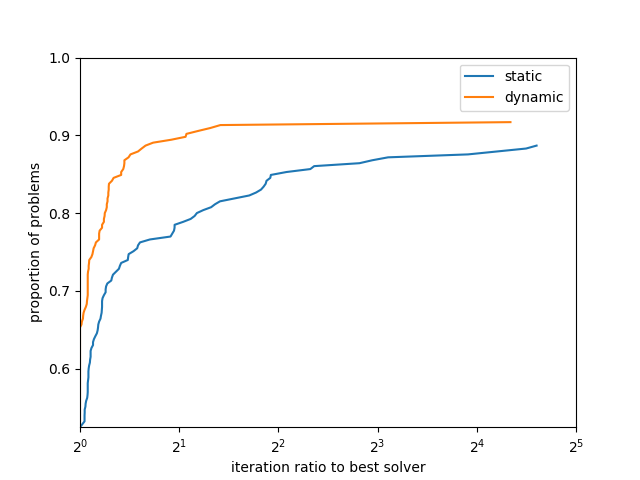
\includegraphics[scale=0.5]{ratios-dynamic-static.png}
%\caption{Comparison of dynamic and static $\mu$ updates for the one-phase algorithm.}
%\end{figure}

In Figure~\ref{fig:ls-options} we trial different line search conditions for the stabilization steps. In particular, we compare the default setting of a `filter' as described in line~\ref{line:filter} of Algorithm~\ref{alg:stable} against other possible conditions. The first baseline to replace this filter condition with  \eqref{phi-sufficient-progress}, i.e., check that sufficient progress is made on the `log barrier' merit function. The other baseline is removing the filter condition entirely and simple taking the maximum step possible. Figure~\ref{fig:ls-options} indicates that the filter has superior performance of these three options.

\begin{figure}[H]
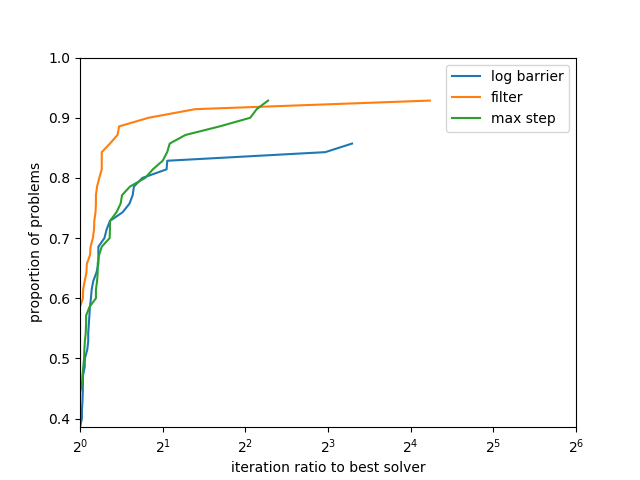
\includegraphics[scale=0.5]{ls-options.pdf}
\caption{Comparison of different line search options.}\label{fig:ls-options}
\end{figure}

In Figure~\ref{fig:num-corrections} we compare different choices of the parameter $c_{\max}$, the maximum number of corrections ($c_{\max}$ is used on line~\ref{take-steps} in Algorithm~\ref{one-phase-IPM}). As one would expect, increasing the number of corrections decreases the iteration count, but has little impact on the failure rate. In the actual implementation of our one-phase algorithm we chose $c_{\max}=3$.
%can see the number of iterations is

\begin{figure}[H]
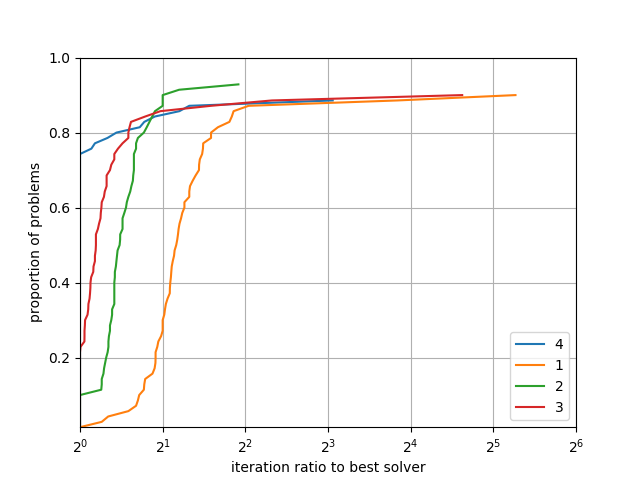
\includegraphics[scale=0.5]{num-corrections.pdf}
\caption{Comparison of the maximum number of corrections for the one-phase algorithm.}\label{fig:num-corrections}
\end{figure}


\begin{figure}[H]
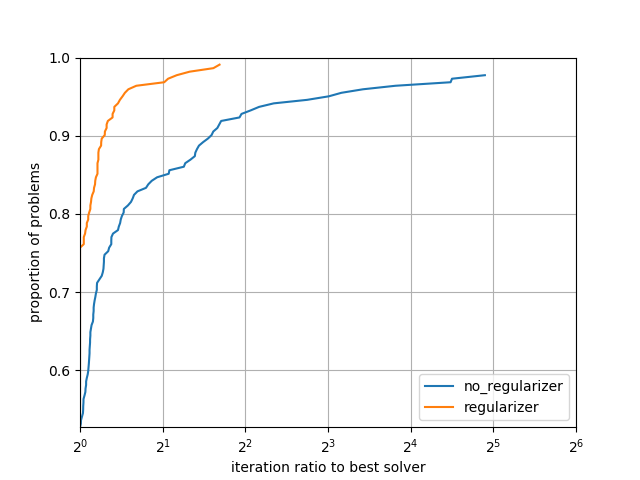
\includegraphics[scale=0.5]{regularizer-ratios.pdf}
\caption{Comparison of the algorithm with and without the regularizer.}\label{fig:num-corrections}
\end{figure}


\subsection{Comparison with IPOPT}\label{alg:comparison-IPOPT}

Please take these results with a grain of salt since we are comparing iteration counts not runtimes.

\todo[inline]{Comparison on number of function/constraint evaluations (clearly admit algorithm is not optimized to minimize constraint violation/function evaluation)}


We consider the final function values $f^{a}_{*}$ and $f^{b}_{*}$ of algorithm $a$ and $b$ respectively approximately the same if:
$$
\frac{f^{a}_{*} - f^{b}_{*}}{1 + \max \{ | f^{a}_{*} |, | f^{b}_{*} | \} } < 10^{-1},
$$
otherwise, we consider the solution of algorithm $a$ better than algorithm $b$ if $f^{a}_{*}  < f^{b}_{*}$. For problems where both algorithm find a KKT point this is reported in the top three rows of Table~\ref{tbl:pairwise-outcomes}. The remainder of Table~\ref{tbl:pairwise-outcomes} shows the number of times both algorithms succeed, fail, or just one algorithm fails. We consider the algorithm to have succeeded if it produces either a certificate of first order local optimality, infeasibility or unboundedness. 

Let us highlight a few interesting facts from the tables. The one-phase algorithm seem to find better KKT points on $13$ problems versus $2$ for IPOPT (Table~\ref{tbl:pairwise-outcomes}). Furthermore, IPOPT fails on $39$ problems compared with $21$ problems for the one-phase algorithm (Table~\ref{tbl:termination-status-counts}). A large proportion of these failures occur before IPOPT has started (Table~\ref{tbl:failure-reasons}).

\begin{table}[H]
\caption{Pairwise comparison of outcomes for IPOPT and the one-phase algorithm}\label{tbl:pairwise-outcomes}
\begin{tabular}{ c c r }
  One Phase &  IPOPT &  \# \\
  \hline
same KKT & - & 158  \\
- & better KKT & 2 \\
better KKT & - &  13 \\
\hline
Succeed & Succeed & 185 \\
Fails & Fails & 7 \\
Succeed & Fails &  32 \\
Fails & Succeed & 14 \\
\end{tabular}
\end{table}

%Table~\ref{tbl:termination-status-counts} displays the 

\begin{table}[H]
\caption{Termination status counts}\label{tbl:termination-status-counts}
\begin{tabular}{ c c c r }
 &  One Phase &  IPOPT &  \\
  \hline
KKT &  201 & 191 \\
unbounded & 4 & 0  \\
primal infeasible & 12 &  8 \\
fail & 21 & 39 \\
\end{tabular}
\end{table}

\begin{table}[H]
\caption{Failure reasons}\label{tbl:failure-reasons}
\begin{tabular}{ c c c r }
 &  One Phase & IPOPT \\
  \hline
max time & 10 & 9  \\
max iter &  3 & 3 \\
error before starting & 4 & 19 \\
error during algorithm & 4 & 8 \\
\hline
total & 21 & 39
\end{tabular}
\end{table}

Figure~\ref{fig:comparison-IPOPT-on-CUTEst} compares the iterations that IPOPT and the one-phase algorithm take to succeed (produce a certificate of first order local optimality, infeasibility or unboundedness) on the CUTEst test set. Note that the iteration counts for the solvers are similar, except that the one-phase solver fails less frequently.


\begin{figure}[H]
\includegraphics[scale=0.5]{ratios-IPOPT-one-phase.pdf}
\includegraphics[scale=0.5]{iterations-IPOPT-one-phase.pdf}
%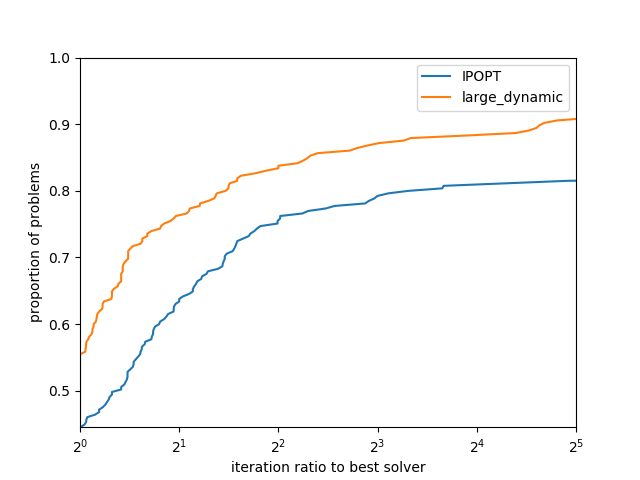
\includegraphics[scale=0.5]{ratios-n=50-10000.png}
%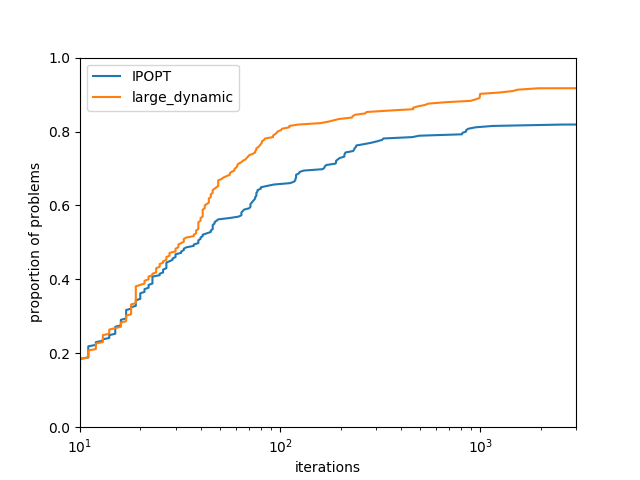
\includegraphics[scale=0.5]{iterations-n=50-10000.png}
\caption{Comparison of IPOPT and one-phase on CUTEst for problems where at least one solver declared the problem optimal, infeasible or unbounded.}\label{fig:comparison-IPOPT-on-CUTEst}
\end{figure}

\todo[inline]{table or plot of maximum dual variables? this would significantly strengthen case.}

\subsection{Comparison on infeasible problems}\label{sec:infeas}

Most of the CUTEst problems have feasible solutions. To generate a test set that was more likely to contain infeasible problems we perturbed the constraints as follows:
$$
\tilde{a}(x) = \cons(x) + e
$$
The solver terminated with the statuses described in the Table~\ref{tbl:termination-status-counts-peturbed}. This test was only run on problems with at most $1,000$ variables and constraints total.
\begin{table}[H]
\caption{Termination status counts for perturbed CUTEst problems.}\label{tbl:termination-status-counts-peturbed}
\begin{tabular}{ c c c r }
 &  One Phase &  IPOPT &  \\
  \hline
KKT & 22 & 20 \\
unbounded & 1 & 0  \\
primal infeasible & 44 &  38 \\
fail & 3 & 12 \\
\end{tabular}
\end{table}

Next, in Figure~\ref{fig:comparison-IPOPT-on-perturbed-CUTEst} we compare IPOPT and the one-phase on the subset problems which at least one solver declared the problem locally infeasible. From this figure one can see that the one-phase solver is quicker and more robust than IPOPT.

\begin{figure}[H]
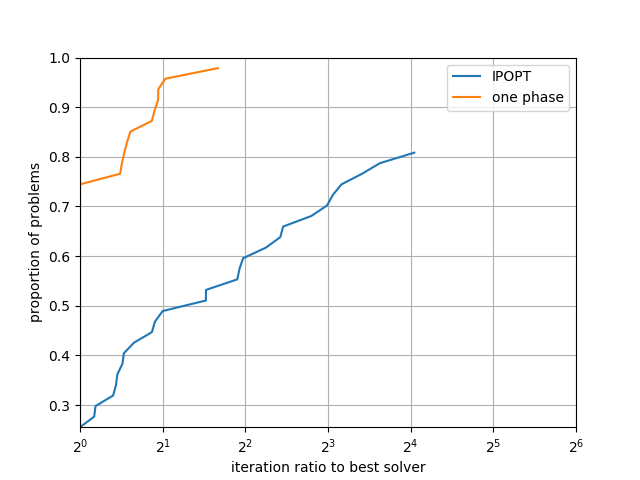
\includegraphics[scale=0.5]{infeas-ratios.png}
\caption{Comparison of IPOPT and one-phase on perturbed CUTEst problems for which at least one solver declares the problem locally infeasible.}\label{fig:comparison-IPOPT-on-perturbed-CUTEst}
\end{figure}

%
%\subsection{Comparison on NETLIB for linear programming}\label{sec:netlib}
%
%The purpose of this Section is to show that the one-phase algorithm has good performance on linear programs, as one would expect since the algorithm is heavily influenced by ideas from linear programming [REF]. My experience from our previous paper is that there is a huge difference in the performance of IPOPT and the one-phase algorithm.
%
%[Use IPOPT option specialized for LP]
%
%\begin{figure}[H]
%\missingfigure{...}
%%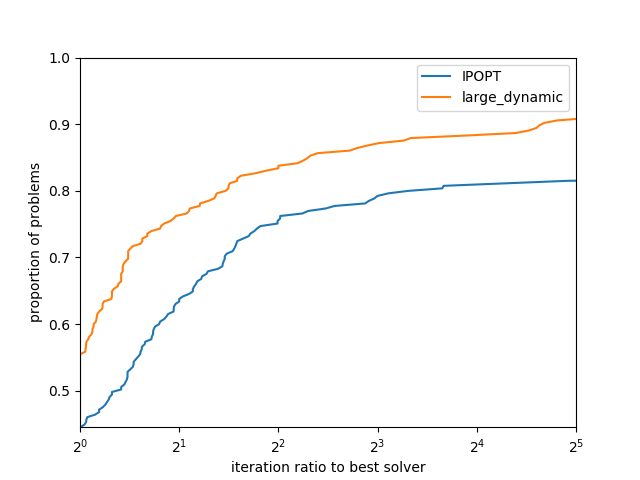
\includegraphics[scale=0.5]{ratios-n=50-10000.png}
%%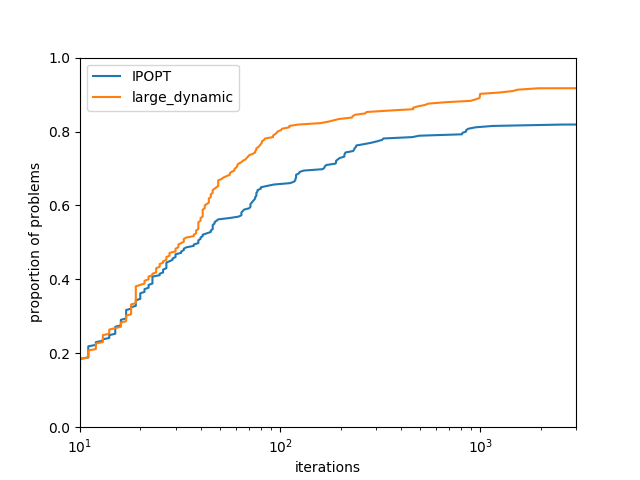
\includegraphics[scale=0.5]{iterations-n=50-10000.png}
%\caption{Comparison of IPOPT and one-phase on the NETLIB linear programming test set.}
%\end{figure}


\section{Conclusions}
\begin{enumerate}
\item ??
\end{enumerate}


\section{To do}

\begin{enumerate}
\item clean up 
\item edit code to match document
\item run full CUTEst test
\item explain performance on Watcher-Beliger example.
\end{enumerate}

\bibliographystyle{abbrvnat} %abbrv}
\bibliography{library-one-phase-2.bib}


\appendix

\section{Global convergence proofs for Algorithm~\ref{one-phase-IPM}}\label{app:global-conv}

\subsection{Convergence of aggressive steps}

\subsubsection{Proof of Lemma~\ref{lem:agg-finite}}\label{sub:lem:agg-finite}

\lemAggFinite*

\begin{proof}
We have
\begin{flalign*}
\| Y \conWeight \|_{\infty} &\le \frac{\max\{ \| \grad \cons(x)^T y \|_{\infty}, \| S y \|_{\infty} \}}{ \TOLinf \min\{  1, \vioVar \}} \\
& \le  \frac{\max\{\| \grad \obj(x) \|_{\infty} + \| \grad \Lag_{\mu} (x , y) \|_{\infty}, \mu / \parComp \}}{ \TOLinf \min\{  1, \vioVar \}} \\
& \le \frac{ 2 G }{ \TOLinf \TOLopt} 
\end{flalign*}
where the first inequality follows from the fact that the \eqref{terminate-primal-infeasible} is not satisfied; the second inequality from the triangle inequality applied to $\| \grad \Lag_{\mu} (x , y) \|_{\infty}$ and inequality \eqref{agg-criteron-buffer}; and the third inequality from inequality \eqref{agg-criteron-farkas} and the Lemma's assumptions.

Next, for any trial step size $\alpha_{P}$ by \eqref{min-step-size-aggresssive} we have
\begin{flalign*}
\alpha_{P} &\ge  \min_{i : w_i > 0}{ \frac{\parBacktracking \theta s_{i}}{2 \vioVar \conWeight_i} }
\ge \min_{i : w_i > 0}{ \frac{ \parBacktracking \theta \parCompAgg}{2 \conWeight_i  y_{i}}  } 
\ge \frac{ \parBacktracking \theta \parCompAgg \TOLinf \TOLopt}{4 G}
\end{flalign*}
where the first inequality is from the minimum trial step size from \eqref{min-step-size-aggresssive}, the second inequality from \eqref{agg-criteron-buffer} and the final inequality from our bound on $\| Y\conWeight\|_{\infty}$.

Therefore we reduce $\mu$ by at least $\alpha_{P} \mu$ each call to Algorithm~\ref{alg:aggressive} that terminates with $\status = \success$. Furthermore,  for sufficiently small $\mu$ whenever \eqref{agg-criteron} holds the optimality criterion \eqref{terminate-kkt} is satisfied. Combining these facts proves the Lemma.
\end{proof}

\subsubsection{Proof of Lemma~\ref{lemma:agg-succeeds}}\label{sec:lemma:agg-succeeds}

\lemAggSucceeds*

\begin{proof}
First, observe that as $\delta \rightarrow \infty$ the direction $d_{x}$ computed from \eqref{eq:schur-complement-system} tends to zero. Consider any $\alpha_{P} \in (0,1)$, since the function $a$ is continuous for sufficiently large $\delta$ we have
\begin{flalign}\label{eq:a-bound}
\| \cons(x) - \cons(x + \alpha_{P} d_{x}) \|_{\infty} \le \frac{\theta}{2} \min\{ s_{i} \}
\end{flalign}
where $\theta$ is defined in equation~\eqref{min-step-size-aggresssive}.

To obtain a contradiction assume that Algorithm~\ref{alg:aggressive} fails. This implies by \eqref{min-step-size-aggresssive} that the backtracking line search of the algorithm will have attempted some $\alpha_{P}$ such that
\begin{flalign}\label{eq:alpha-bound}
\alpha_{P} \in \left[ 0, \min_{i : w_i > 0}{ \frac{\theta s_{i}}{2 \vioVar \conWeight_i} }  \right], %\frac{1}{1 + (\vioVar / (  \parCompAgg \mu) ) \| y \|_{\infty}}\right]
\end{flalign}
then for this choice of $\alpha_{P}$ we have
$$
\| s^{+} - s \|_{\infty} = \|  -\alpha_{P} \mu\conWeight+  \cons(x) - \cons(x + \alpha_{P} d_{x}) \|_{\infty} \le  \alpha_{P} \mu \|  \conWeight \|_{\infty} +  \| \cons(x) - \cons(x + \alpha_{P} d_{x}) \|_{\infty} \le \theta \min_i\{ s_{i} \},
$$
where the first equality holds by \eqref{eq:slackVarUpdate} and final inequality holds by \eqref{eq:a-bound} and \eqref{eq:alpha-bound}.
Since $\theta \le 1 - \parFracBoundary$ the fraction to the boundary rule~\eqref{fracBoundary-primal} is satisfied. Note that using the definition of $\theta$ from \eqref{min-step-size-aggresssive} and that $\parComp < \parCompAgg$ we get
$$
\frac{s^{+} Y}{\mu} \in [\parComp / \parCompAgg, \parCompAgg / \parComp]  \frac{s Y}{\mu} \subseteq  [\parComp, 1/\parComp ] e
$$
therefore $\alpha_{D} = 0$ gives a feasible dual iterate. We obtain a contradiction, because the step should have been accepted.
\end{proof}

\subsection{Convergence results for stabilization steps}

\subsubsection{Proof of Lemma~\ref{lem:compact-Q}} \label{sec:lem:compact-Q}

Note that during Lemma~\ref{lem:compact-Q} we will repeatedly use that the following elementary real analysis fact: 

\begin{fact}
If $g_i$ is a continuous function and the set $X = \{ x : g_i(x) \le 0 \}$ is bounded, then the set $X$ is compact
\end{fact}

\lemCompactQ*

\begin{proof}
First consider the set
$$
Q := \left\{ x \in \R^{\nvar} : (y, s) \in \R^{\ncon++} \times \R^{\ncon++}, \phi_{\mu}(x,y,s) \le C, \| \max\{ \cons(x), e \} \|_{\infty} \ge \max\{1,-\obj(x) \} \TOLunbounded \right\} 
$$
Now, consider some $x \in Q$. Recall that
$$
\phi_{\mu}(x, s, y) = \obj(x) + \mu \left( \parRegularizer \sum_{i = 1}^{\nvar} \sqrt{x_i^2 + 1 / \parRegularizer^2} - \parConRegularizer e^T \cons(x) \right)  - \mu  \sum_i{ \log \left( \vioVar \conWeight_i - a_i(x)  \right) } + \frac{\| S y - \mu \|_{\infty}^3}{\mu^2}.
$$
The expression $\parConRegularizer a_i(x) - \log(\mu \conWeight_i - a_i(x))$ and $\frac{\| S y - \mu \|^3}{\mu^2}$ are bounded from bellow. Therefore there exists some constant $K_{1} > 0$ such that
$$
-K_{1} \le \obj(x) \le K_{1} - \parRegularizer \sum_{i}{\sqrt{x_i^2 + 1 / \parRegularizer^2}}
$$
It follows that $x$ is bounded and therefore $Q$ is bounded. Furthermore, since $\phi_{\mu}(x) \le C$ and $Q$ is bounded there exists some constant $K_{2} > 0$ such that
$$
\mu w - \cons(x) \ge K_{2}
$$
for all $x \in Q$. Consider some sequence $x^{k} \in Q$ with $x^{k} \rightarrow x^{*}$. The statement $\cons(x) \le \mu w - K_{2}$ implies $\phi_{\mu}$ is continuous in a neighborhood of $x^{*}$. Using the definition of $Q$ and the assumption that $f$ and $a$ are continuous implies $x^{*} \in Q$, i.e., $Q$ is compact. 


%Using the fact that $Q$ is compact and $s > 0$ we deduce that $S^{-1} e$ is bounded, it follows that
Note that:
$$
\mathbb{Q}_{\mu, C} = \left\{ (x,y,s) \in \R^{\nvar} \times \R^{\ncon++} \times \R^{\ncon++} : x \in Q, \cons(x) + s = \mu \conWeight, \frac{S y}{\mu} \in [\parComp e, e / \parComp]\right\}.
$$
Consider some $(x,y,s) \in \mathbb{Q}_{\mu, C}$, since $s = \mu w - \cons(x) \ge K_{2}$ and $\frac{S y}{\mu} \in [\parComp e, e / \parComp]$ we can deduce $y$ is bounded. Since the function $\cons(x)$ and $S y$ are continuous we conclude $\mathbb{Q}_{\mu, C}$ is compact.
\end{proof}

\begin{restatable}{corollary}{coroBoundEverything}\label{coro:bound-everything}
Let the functions $f : \R^{\nvar} \rightarrow \R$ and $a : \R^{\nvar} \rightarrow \R^{\ncon}$ be twice differentiable. Consider some fixed $\mu > 0$.
Then there exists some $L > 0$ such that for all $(x, s, y) \in \mathbb{Q}_{\mu, C}$ the following inequalities hold:
$$
s_i, y_i \ge 1/L
$$
$$
\| x \|, \| y \|, \| s \|, \| \grad \barrier_{\mu}(x) \|, \| \schur \|, \| \grad \cons(x) \| \le L
$$
and for any $d$ s.t. $\| d \| < 1 / L$
\begin{subequations}\label{lipschitz-continuous}
\begin{flalign}
\barrier_{\mu}(x + d) &\le \barrier_{\mu}(x) + \grad \barrier_{\mu}(x)^T d + L / 2 \| d \|^2 \label{phi-lipschitz-continuous} \\
\| \cons(x + d) - \cons(x) \| &\le L  \| d \|. \label{a-lipschitz-continuous}
\end{flalign}
\end{subequations}

Furthermore, if the aggressive criterion~\eqref{agg-criteron} does not holds:
$$
\max\{ \| \grad \barrier_{\mu}(x) \|, \| S y - \mu \|_{\infty} \} \ge 1 / L
$$
\end{restatable}

\begin{proof}
All these claims use Lemma~\ref{lem:compact-Q} and the elementary real analysis fact that for any continuous function $g$ on a compact set there $X$ there exists some $x_{*} \in X$ such that $g(x_{*}) = \sup_{x \in X}{g(x)}$.

The only non-trivial claim is showing \eqref{lipschitz-continuous}, which proceed to show. Since there exists some constants $\varepsilon_{1} > 0$ such that $(x,y,s) \in \mathbb{Q}_{\mu, C}$ we have $\cons(x) \le \mu w - \varepsilon_{1}$. It follows that there exists some constant $\varepsilon_2 > 0$ such that for all $\| d \| \le \varepsilon_2$ we have $\cons(x + d) < \mu w$. It follows that there exists some $L > 0$ such that $\| \grad^2 \barrier_{\mu}(x) \| \le L$.

For some $x$ and $\nu$ with $\| \nu \| = 1$ define the one dimensional function
$$
h(\alpha) :=  \barrier_{\mu}(x + \alpha \nu) 
$$
then for $\alpha \in [0, \varepsilon_2]$ we get
$$
h(\alpha) - h(0) - \alpha h'(0) = \int_{0}^{\alpha}{ \int_{0}^{\eta_{2}}{h''(\eta) \partial \eta_{1} \partial \eta_{2}} } \le \alpha^2 L / 2,
$$
which using $d = \nu \alpha$ for $\alpha \in [0, \varepsilon_2]$ concludes the proof of \eqref{phi-lipschitz-continuous}. Showing \eqref{a-lipschitz-continuous} consists of a simpler version of the argument for \eqref{phi-lipschitz-continuous}.
\end{proof}

With Corollary~\ref{coro:bound-everything} in hand we proceed to showing for sufficiently large $\delta$, Algorithm~\ref{alg:stable} will succeed.
%that there will only be a finite number of stabilization steps until the next aggressive step.


\subsubsection{Proof of Corollary~\ref{coroConsecutiveStable}}\label{sec:coroConsecutiveStable}

Using Lemma~\ref{lem:stable-succeed-for-large-delta} we can prove Corollary~\ref{sec:coroConsecutiveStable}. Lemma~\ref{lem:stable-succeed-for-large-delta} states that

\begin{restatable}{lemma}{lemStableSucceedForLargeDelta} \label{lem:stable-succeed-for-large-delta}
Let the functions $f : \R^{\nvar} \rightarrow \R$ and $a : \R^{\nvar} \rightarrow \R^{\ncon}$ be twice differentiable. There exists some $\bar{\delta} > 0$ such that for any $(x,y,s) \in \mathbb{Q}_{\mu,C}$ and $\delta \in [\bar{\delta}, \infty)$ the following statement holds. If Algorithm~\ref{one-phase-IPM} calls Algorithm~\ref{alg:stable} on the first inner iteration at the point $(\mu, x, s, y)$, then Algorithm~\ref{alg:stable}  terminates with $\status = \success$.
\end{restatable}

The proof of Lemma~\ref{lem:stable-succeed-for-large-delta} is deferred to Section~\ref{sec:lem:stable-succeed-for-large-delta}.

\coroConsecutiveStable*

\begin{proof}
Suppose in order to obtain a contradiction there is a infinite sequence of consecutive stabilization steps. Then there are two possibilities (i) there is an infinite sequence of consecutive steps where the sufficient decrease in the augmented log barrier function \eqref{phi-sufficient-progress} is satisfied or (ii) there is an infinite subsequence of stabilization steps where a sufficient decrease in the KKT error \eqref{eq:kkt-progress} is satisfied.

Since the unboundedness termination criterion~\eqref{terminate-dual-infeasible} is not met, we know by Lemma~\ref{lem:compact-Q} there exists some compact set $\mathbb{Q}_{\mu,C}$ that contains all the iterates.

Consider case (i). Consider any $\bar{\delta} > 0$ as defined in Lemma~\ref{lem:stable-succeed-for-large-delta}. Lemma~\ref{lem:stable-succeed-for-large-delta} implies a step will be taken with $\delta \le \parDeltaIncreaseFailure \bar{\delta}$. Now, consider any such step $(x,y,s)$ to $(x^{+}, s^{+}, y^{+})$ with step size $\alpha_{P}$. Using that the aggressive criterion~\eqref{agg-criteron} is not satisfied and that $\| \schur(\mu, x, s, y) \|$ is bounded on the compact set $\mathbb{Q}_{\mu,C}$, we deduce there exists some constant $K > 0$ such that $\tilde{\Delta}^{\phi_{\mu}}_{(x,y)}(\alpha_{P} d_{x}, \alpha_{P} d_{y}) < K$ for all $\delta \le \parDeltaIncreaseFailure \bar{\delta}$ and $\alpha_{P} > \parMinStableStepSize$ \todo{moves a little to quick}. Since the criterion for sufficient progress on the augmented log barrier function \eqref{phi-sufficient-progress} is satisfied, we deduce there exists some constant $K > 0$ such that $\phi_{\mu}(x^{+}, s^{+}, y^{+}) \le \phi_{\mu}(x, s, y) - K$ at each iteration, which implies eventually the unboundedness criterion~\eqref{terminate-dual-infeasible} is met. 

Consider case (ii). Since \eqref{eq:kkt-progress} holds for an infinite subsequence $(x^{k}, y^{k}, s^{k})$ and $\alpha_{P} > \parMinStableStepSize$ by \eqref{eq:min-step-size-stable} we have $K_{\mu}(x^{k}, y^{k}, s^{k}) \rightarrow 0$. This implies eventually the aggressive criterion~\eqref{agg-criteron} is met.

Therefore neither case (i) or (ii) is possible. By contradiction the result holds.
\end{proof}


\subsubsection{Proof of Lemma~\ref{lem:stable-succeed-for-large-delta}}\label{sec:lem:stable-succeed-for-large-delta}

Before we prove Lemma~\ref{lem:stable-succeed-for-large-delta} we prove two sub-lemmas.

\begin{restatable}{lemma}{lemLogBarrierLargeDelta} \label{lem:log-barrier-large-delta}
Let the functions $f : \R^{\nvar} \rightarrow \R$ and $a : \R^{\nvar} \rightarrow \R^{\ncon}$ be twice differentiable. Consider any fixed $\mu > 0$.
There exists some $c_{1}, c_{2}, \bar{\delta} > 0$ such that for any $(x,y,s) \in \mathbb{Q}_{\mu,C}$ and $\delta \in [\bar{\delta}, \infty)$ the following statement holds. If Algorithm~\ref{one-phase-IPM} calls Algorithm~\ref{alg:stable} on the first inner iteration at the point $(\mu, x, s, y)$, then the computed direction satisfies 
$$
\barrier_{\mu} (x + d_{x}) \le \barrier_{\mu} (x) + \parObjReductFactor \tilde{\Delta}^{\barrier_{\mu}}_{(x,y)}( d_{x} ) - c_1 \| \grad \barrier_{\mu} (x) \|^2
$$
%and if $\delta \in [0, \parDeltaIncreaseFailure \bar{\delta}]$ then:
%$$
% \tilde{\Delta}^{\barrier_{\mu}}_{(x,y)}( \alpha_{P} d_{x} ) \le -c_{2} \| \grad \barrier_{\mu}(x) \|^2
%$$
\end{restatable}



\begin{proof}
Recall the matrix $\schur$ as defined in \eqref{eq:schur-matrix}.

Consider some $c_{2} \in (\parObjReductFactor, 1)$ then there exists some constant $C > 0$ such that for all $\delta$ greater than
$C \left( \| \schur \| + \| \grad \barrier_{\mu}(x) \| \right)$, we have:
\begin{flalign}\label{eq:C-big-enough}
 \lambda_{\min}  / \lambda_{\max} \le \sqrt{c_{2}}, 1 - L \lambda_{\max} / \lambda_{\min}^2 \ge \sqrt{c_{2}}, \| d_{x} \| < 1 / L
\end{flalign}
where $\lambda_{\min}$ and $\lambda_{\max}$ denote the smallest and largest eigenvalues of the matrix $H = \schur + \delta I$.


Now,
\begin{flalign*}
\barrier_{\mu}(x + d_{x}) - \barrier_{\mu}(x) - \frac{\parObjReductFactor}{2} d_{x}^T \schur d_{x}
&\le_{(i)}   \grad \barrier_{\mu}(x)^T d_{x} + L \| d_{x} \|^2 \\
 &=_{(ii)} -\grad \barrier_{\mu}(x)^T H^{-1} \grad \barrier_{\mu}(x) + L  \grad \barrier_{\mu}(x)^T H^{-2} \grad \barrier_{\mu}(x) \\
  &\le_{(iii)} -\| \grad \barrier_{\mu}(x) \|^2 / \lambda_{\max} (1  - L \lambda_{\max} /  \lambda_{\min}^2) \\
  &\le_{(iv)} -c_{2} \| \grad \barrier_{\mu}(x) \|^2 / \lambda_{\min} \\
  &=_{(v)} -\parObjReductFactor  \| \grad \barrier_{\mu}(x) \|^2 / \lambda_{\min} - (c_{2} - \parObjReductFactor) / \lambda_{\min} \| \grad \barrier_{\mu}(x) \|^2  \\
    &\le_{(vi)}  - \parObjReductFactor \grad \barrier_{\mu}(x)^T H^{-1} \grad \barrier_{\mu}(x) - (c_{2} - \parObjReductFactor)  / \lambda_{\min}   \| \grad \barrier_{\mu}(x) \|^2 \\
    &=_{(vii)}  - \parObjReductFactor \grad \barrier_{\mu}(x)^T d_{x} - (c_{2} - \parObjReductFactor)  / \lambda_{\min}   \| \grad \barrier_{\mu}(x) \|^2 \\
\end{flalign*}
where:
\begin{enumerate}[label=(\roman*)]
\item holds by Corollary~\ref{coro:bound-everything} and equation~\eqref{eq:C-big-enough}
\item using $H d_{x} = -\grad \barrier_{\mu}(x)$
\item $\| v \|^2 / \lambda_{\min} \ge v^T H^{-1} v \ge \| v \|^2 / \lambda_{\max}$ for any $v$
\item By equation~\eqref{eq:C-big-enough}
\item Expanding
\item $\| v \|^2 / \lambda_{\min} \ge v^T H^{-1} v $ for any $v$.
\item using $H d_{x} = -\grad \barrier_{\mu}(x)$
\end{enumerate}

Since $\frac{c_{2} - \parObjReductFactor}{\lambda_{\min}} > 0$, we have proved the claim.
\end{proof}

\begin{restatable}{lemma}{lemCompLargeDelta} \label{lem:comp-large-delta}
Let the functions $f : \R^{\nvar} \rightarrow \R$ and $a : \R^{\nvar} \rightarrow \R^{\ncon}$ be twice differentiable. Consider any fixed $\mu > 0$
and $c_{1} > 0$. There exists some $\bar{\delta} > 0$ such that for any $(x,y,s) \in \mathbb{Q}_{\mu,C}$ and $\delta \in [\bar{\delta}, \infty)$ the following statement holds. If Algorithm~\ref{one-phase-IPM} calls Algorithm~\ref{alg:stable} on the first inner iteration at the point $(\mu, x, s, y)$, then the computed direction and trial point $(x^{+}, y^{+}, s^{+}, \mu)$ corresponding to $\alpha_{P} = 1$ satisfies
%a new point $(x^{+}, s^{+}, y^{+})$ with:
\begin{flalign}
s + d_{s} &\ge \parFracBoundaryMax s \label{eq-lem:frac-boundary-max} \\
s^{+} &\ge  \parFracBoundary s \label{eq-lem:frac-boundary} \\
S^{+} y^{+} &\in [\mu e \parComp, \mu e/\parComp] 
\end{flalign}
Furthermore,
$$
\MeritComp(x^{+},y^{+}) \le \MeritComp(x,y) +  \parObjReductFactor \tilde{\Delta}^{\MeritComp}_{(x,y)}( d_{x}, d_{y} ) + \left( c_{1} -  \MeritComp(x,y) (1 - \parObjReductFactor) \right)
$$
\end{restatable}

\begin{proof}
Consider any $\gamma \in (0,1)$ and define
$$
\bar{\delta}_{2}(x,s,y) = \lambda_{\min} ( \schur ) + 1 / \gamma
$$
Let $q( x, s, y)$ be some function $q : \mathbb{Q}_{\mu,C} \rightarrow \R$  and recall $\mu > 0$ is fixed.
We use the notation $q = O(\gamma)$ to denote that there exists some constant $K > 0$ such that  $q(x, s, y) \le K \gamma$ each time Algorithm~\ref{one-phase-IPM} calls Algorithm~\ref{alg:stable} on the first inner iteration.


Then for any $\delta \ge \bar{\delta}_{2}(x,s,y)$ we have:
$$
\| d_{x} \| = O(\gamma)
$$
Hence by Corollary~\ref{coro:bound-everything} we have:
\begin{flalign*}
\| S^{-1} d_{s}  \|_{\infty} = O( \gamma ) \\
\| S^{-1} (S^{+} - S)  \|_{\infty} = O( \gamma ) 
\end{flalign*}
which for sufficiently small $\gamma$ implies \eqref{eq-lem:frac-boundary-max} and \eqref{eq-lem:frac-boundary}.

Furthermore,
\begin{flalign*}
\| Y^{-1} d_{y} \|_{\infty} &= \| \mu  (Y S)^{-1}  e - e + S^{-1} d_{s}  \|_{\infty} \\
&\le (1 / \parComp - 1) + \| S^{-1} d_{s}  \|_{\infty} \le 1 / \parComp + O(\gamma)
\end{flalign*}
Therefore:
\begin{flalign*}
\| \mu - S^{+} y^{+} \|_{\infty} &\le \| \mu - S^{+} (y + d_{y}) \|_{\infty} \\
 &\le \| \mu - S (y + d_{y}) \|_{\infty}  +  \| (S - S^{+}) (y + d_{y}) \|_{\infty} \\
 &=  \| Y d_{s} \|_{\infty} +  \| (S - S^{+}) (y + d_{y}) \|_{\infty} \\
 &= O(\gamma)
\end{flalign*}
Where the first inequality follows from $\alpha_{P} = 1$ from \eqref{eq:alphaD-least-squares} and the second inequality by the triangle inequality, the third by $\mu - S y + S d_{y} + Y d_{s} = 0$ and the fourth by $\| s - s^{+} \| = O(\gamma)$ and $\| d_{s} \| = O(\gamma)$. Hence

$$
\MeritComp(x^{+},y^{+}) = \frac{\| \mu - S^{+} y^{+} \|_{\infty}^3 }{\mu^2} = O( \gamma^3 ).
$$
Since:
$$
\MeritComp(x,y) +  \tilde{\Delta}^{\MeritComp}_{(x,y)}( d_{x}, d_{y} ) = 0
$$
the result holds.
\end{proof}


\lemStableSucceedForLargeDelta*

\begin{proof}
There exists some $c_{2} > 0$ such that 
$$
c_{2} -  \MeritComp(x,y) / 2 - c_{1} \| \grad \barrier_{\mu} (x) \|^2 \le 0
$$
for all $(x, s, y) \in \mathbb{Q}_{\mu,C}$. Combining Lemmas~\ref{lem:log-barrier-large-delta} and \ref{lem:comp-large-delta} we conclude that there exists some $\bar{\delta}$ such that for all $\delta \ge \bar{\delta}$
\begin{flalign}
\tilde{\Delta}^{\phi_{\mu}}_{(x,y)}(u, v) = \tilde{\Delta}^{\barrier_{\mu}}_{(x,y)}( u ) +   \tilde{\Delta}^{\MeritComp}_{(x,y)}( u, v ).
\end{flalign}

\end{proof}


\section{Matrix factorization strategy}

This strategy is based on the ideas of IPOPT \cite[Algorithm IC]{wachter2006implementation}.

\begin{algorithm}[H]
\textbf{Input:} The matrix $\mathcal{K}_{0}$ and current delta choice $\delta$ \\
\textbf{Output:} The factorization $\mathcal{K}_{\delta}^{-1}$ for some $\delta > 0$ such that the matrix $\mathcal{K}_{\delta}$ has the correct inertia.
\begin{enumerate}[label*=A.{\arabic*}]
\item Set $\delta_{\text{prev}} \gets \delta$
\item Set $\delta \gets 0$
\item Perform LDL factorization of $\mathcal{K}_{\delta}$, if inertia is correct return $\mathcal{K}_{\delta}^{-1}$ otherwise continue.
\item If $\delta_{prev} > 0$ set $\delta \gets \max\{ \parDeltaMin, \delta_{\text{prev}} / 3 \}$ otherwise set $\delta = \delta_{\text{start}} \mu$.
\item Perform LDL factorization of $\mathcal{K}_{\delta}$, if inertia is correct return $\mathcal{K}_{\delta}^{-1}$ otherwise continue.
\item Set $\delta \gets 8 \delta$. Go to previous step.
\end{enumerate}
\caption{Matrix factorization strategy}\label{alg:mat-fact}
\end{algorithm}

\section{The (non-existence) of a central path in non-convex optimization}\label{app:non-existence-of-central-path}

Would be nice to have a long discussion on this issue

$$
f_{\mu}(x) = 50 (x - 0.5)^3 + x - \mu (\log(x) + \log(1 - x))
$$

$$
\grad f_{\mu}(x) = 150.0 * (x - 0.5)^2 + 1.0  - \mu / x + \mu / (1 - x) = 0 \\
$$
Is discontinuous at $\mu = 3$, $x \approx 0.5$, i.e., there exists no function $x(\mu)$ such that $\grad f_{\mu}(x(\mu)) = 0$ and $x(\mu)$ is continuous. 

[Vanderbei' s example for the problem $\min{ x -x^2}$ s.t. $x \ge 0$ there exists no continuous central path from an initial point to the optimal solution. However, optimal solution is unbounded.]


\end{document}